\documentclass[10pt,pdftex]{amsart}
%%=============================
%% Used packages
%%=============================

%%Document Style
\usepackage{a4}
\usepackage[pdftex,pagebackref,colorlinks]{hyperref}
%\usepackage{url}
%%Font Coding
\usepackage[T1]{fontenc}
%%Text Coding
\usepackage[ansinew]{inputenc}
%%Language
\usepackage[english]{babel}
%%AMS Packages
\usepackage{amssymb}
\usepackage{amsthm}
%Graphics
\usepackage[pdftex]{graphicx}
\usepackage[pdftex]{color}
\usepackage{pict2e}
\usepackage[all]{xy}
%Special Environments
\usepackage[vflt]{floatflt}
\usepackage{enumerate}
\usepackage{longtable}
\usepackage{fancyvrb}


%%=============================
%% Defined Environments
%%=============================
\theoremstyle{plain}
\newtheorem{theorem}{Theorem}[section]
\newtheorem{proposition}[theorem]{Proposition}
\newtheorem{lemma}[theorem]{Lemma}
\newtheorem{corollary}[theorem]{Corollary}
\theoremstyle{definition}
\newtheorem{definition}[theorem]{Definition}
\newtheorem{exercise}{Exercise}
\theoremstyle{remark}
\newtheorem*{remark}{Remark}
\newtheorem*{remarks}{Remarks}
\newtheorem*{example}{Example}
\newtheorem*{warning}{WARNING}
\newtheorem*{algorithm}{\textsc{Algorithm}}


%for non fragile code, e.g. without _\%
\def\code{\texttt}
%for fragile inline code use: \verb""
%for paths use \path{}

%paragraphed code
\DefineVerbatimEnvironment{pcode}{Verbatim}{fontsize=\footnotesize,frame=lines,framesep=2ex,xleftmargin=1.5em}
%paragraphed code with line numbering (it is possible to give a line a label with: \label{..} after the line as usual)
\DefineVerbatimEnvironment{pcoden}{Verbatim}{commandchars=\\\{\},fontsize=\footnotesize,numbers=left,numbersep=0.5em,frame=lines,framesep=2ex,xleftmargin=1.5em}
%Above environments are to be used as normal, i.e. \begin{pcode}\end{pcode} or \begin{pcoden}\end{pcoden}

%paragraphed code from file
\CustomVerbatimCommand{\inputcode}{VerbatimInput}{fontsize=\footnotesize,frame=lines,framesep=2ex,xleftmargin=1.5em}
%paragraphed code from file with line numbering
\CustomVerbatimCommand{\inputcoden}{VerbatimInput}{fontsize=\footnotesize,numbers=left,numbersep=0.5em,frame=lines,framesep=2ex,xleftmargin=1.5em}
%Above commands are to be used as normal, i.e. \inputcode{dir/file.ext} or \inputcoden{dir/file.ext}


%%=============================
%% Counters
%%=============================
\numberwithin{equation}{section}
\numberwithin{figure}{section}
\numberwithin{exercise}{section}
\renewcommand\theenumi{\roman{enumi}}


%%=============================
%% Defined Math Operators
%%=============================

\DeclareMathOperator{\card}{card}
\DeclareMathOperator{\conv}{conv}
\DeclareMathOperator{\diam}{diam}
\DeclareMathOperator{\dist}{dist}
\DeclareMathOperator{\ddiv}{div}
\DeclareMathOperator{\esup}{ess \sup}
\DeclareMathOperator{\im}{Im}
\DeclareMathOperator{\interior}{int}
\DeclareMathOperator{\sgn}{sgn}
\DeclareMathOperator{\supp}{supp}
\DeclareMathOperator{\vol}{vol}
\DeclareMathOperator{\grad}{\nabla}


%%=============================
%% Defined Abreviations
%%=============================

\def\FFW{{\rm \kern-.08em{F}\kern-.15em\lower.3ex\hbox{\tiny{F}}\kern-.1em \lower-.1ex\hbox{\footnotesize{W}}} }

%%Spaces
\def\C{\ensuremath{\mathbb{C}}}
\def\Cinv{\ensuremath{\C^{-1}}}
\def\R{\ensuremath{\mathbb{R}}}


%%Colors
%\definecolor{string}{rgb}{0.7,0.0,0.0}


\title{\FFW Documentation}
\author[Byfut]{A. Byfut}
\author[Gedicke]{J. Gedicke}
\author[G\"unther]{D. G\"unther}
\author[Mellmann]{H. Mellmann}
\author[Reininghaus]{J. Reininghaus}
\author[Wiedemann]{S. Wiedemann}

\hypersetup{
pdftitle = {FFW Documentation},
pdfsubject = {Finite Elements},
pdfauthor = {A. Byfut, J. Gedicke, D. G\"unther, H. Mellmann, J. Reininghaus, S. Wiedemann},
pdfkeywords = {FEM},
pdfcreator = {pdflatex},
pdfproducer = {}
}


\begin{document}
\maketitle
\tableofcontents
\pagebreak

\section{Introduction}

\noindent This document describes how to use and extend the \textbf{F}inite
element \textbf{F}rame \textbf{W}ork, from here on referred to as
\FFW. The goal of this software package is to provide our target
audience, students and researchers in the field of finite element
research, a tool which presents various methods in a reference
implementation and to provide a platform for future research and development. The
following design goals guided the development decisions:
\begin{itemize}
    \item{Clean and readable implementation precedes performance}
    \item{Good extensibility}
    \item{Easy to debug}
    \item{Providing mechanisms for interpreting and visualizing the numerical results}
\end{itemize}
Following these design goals we have chosen the MATLAB programming
language, as it is relatively wide known in our target audience and
provides a coherent setting in which one can focus on the problem at
hand. For simplicity we only consider methods with triangular
elements in $2D$. The \FFW currently features:
\begin{itemize}
    \item{Methods}
        \begin{itemize}
            \item{$P_1$-$FEM$, a standard conforming discretization for elliptic PDE's}
            \item{$CR$-$FEM$, a non-conforming discretization for elliptic PDE's}
            \item{$RT_0$-$P_0$-MFEM, a mixed FEM for elliptic PDE's}
            \item{$P_1\times P_1$, a standard conforming discretization for elasticity problems}
            \item{$P_1\times CR$, a non-conforming and locking free discretization for elasticity problems}
            \item{$AW$, a mixed, higher order, locking free FEM for elasticity problems}
        \end{itemize}
    \item{Adaptivity}
        \begin{itemize}
            \item{A newest vertex bisection like algorithm for edge oriented mesh refinement that produces shape regular, nested triangulations with no hanging nodes}
            \item{Graded meshes using the above algorithm}
            \item{Reliable and efficient a posteriori error estimators for almost all of the above methods}
            \item{Two marking strategies, maximum and bulk, controlling the mesh refinement based on a posteriori error estimators}
        \end{itemize}
    \item{A global data structure containing all computed data, including complete mesh information like edge enumeration, normals, tangents, etc.}
    \item{A simple reference multigrid implementation for $P_1$-FEM}
    \item{Simple integration routines for efficient calculation of boundary integrals, error norms, etc.}
    \item{Automatic problem creation to reliably test new methods using symbolic differentiation}
    \item{A general framework for output routines to analyse the methods and results}
    \item{Various test problems to illustrate performance of adaptivity and test correctness}
    \item{Full scriptability for automatic computation with different parameters}
\end{itemize}

\section{Quick Start}
\label{sect:QuickStart}
\subsection{Getting Started with the FFW}
\label{sect:QuickStart:gettingStarted}

\noindent This subsection will describe how to execute an existing script for a problem and how to manipulate it.\medskip

\noindent In the following we are interested in the solution $u$ of the elliptic PDE
\begin{align*}
- \ddiv (\kappa \,\grad u) + \lambda \,\grad u + \mu \, u &= f &&\text{in } \Omega,\\
u &= u_D &&\text{on } \Gamma,\\
\frac{\partial u}{\partial n} &= g &&\text{on } \partial\Omega \setminus \Gamma.
\end{align*}
As model problem we consider the above problem with $\kappa = I$, $\lambda = 0$, $\mu = 0$, $f \equiv 1$, $u_D \equiv 0$ and $g \equiv 0$, on a L-shaped domain $\Omega$ with Dirichlet boundary only (Neumann boundary $\partial\Omega \setminus \Gamma = \emptyset$).\medskip

\noindent The script \code{gettingStarted.m} in the root folder shows the basic usage of the \FFW\!. It's code is printed in Figure~\ref{sect:Quickstart.fig.code:gettingStarted}.

\begin{figure}[ht!]
%\inputcoden{../gettingStarted.m}
\begin{pcoden}
function p = gettingStarted

problem = 'Elliptic_Lshape';
pdeSolver = 'P1';
maxNrDoF = 100;
mark = 'bulk';

p = initFFW(pdeSolver,problem,mark,maxNrDoF,'elliptic');
p = computeSolution(p);

figure(1);
set(gcf,'Name','Displacement');
p = show('drawU',p);
view(-30,20)

figure(2);
set(gcf,'Name','Estimated Error');
p = show('drawError_estimatedError',p);
\end{pcoden}

\caption{Content of \code{gettingStarted.m}}\label{sect:Quickstart.fig.code:gettingStarted}
\end{figure}

\medskip
\noindent To start the script, set MATLAB's current directory to the root of the \FFW and execute it.\medskip

\noindent 
\begin{enumerate}[{\hspace{15mm}}]
\item[Line 3:] The name of a file that describes the problem definition. This file is located at \path{.\problems\elliptic\}. For more details on the geometry refer to Section~\ref{sect:DataStructures}. For more details on the problem definition see also Subsection~\ref{sect:QuickStart:ProblemDefinition}.
\item[Line 4:] The type of finite element method is chosen. This can possibly also be \code{'CR'}.
\item[Line 5:] This is the indicator when to stop the refinement, i.e., the calculations. For more details refer to Section~\ref{sect:MeshGeneration}.
\item[Line 6:] The mark algorithm is chosen. The argument can also be \code{'maximum'} or \code{'uniform'}. For more details refer to Section~\ref{sect:MeshGeneration}.
\item[Line 8:] The \FFW is initialized with the above arguments, i.e., the structure \code{p} is created. The last argument describes what problem type is to be computed. This argument can possibly also be \code{'elasticity'}. See also Section~\ref{sect:ImplementedProblems}.
\item[Line 9:] The actual calculations are started. See also Section~\ref{sect:FlowChart} for details.
\item[Line 12:] The solution is plotted with the standard parameters. More details about the \code{show} function as well as its parameters can be found in Section~\ref{sect:GraphicalOutput}.
\item[Line 15:] The estimated error is plotted with the standard parameters.
\end{enumerate}
\bigskip

\noindent For the results, i.e. the solution and the estimated error, of the \code{gettingStarted.m} script, see Figure~\ref{sect:Quickstart.fig.plots.gettingStarted}.

\begin{figure}[ht!]
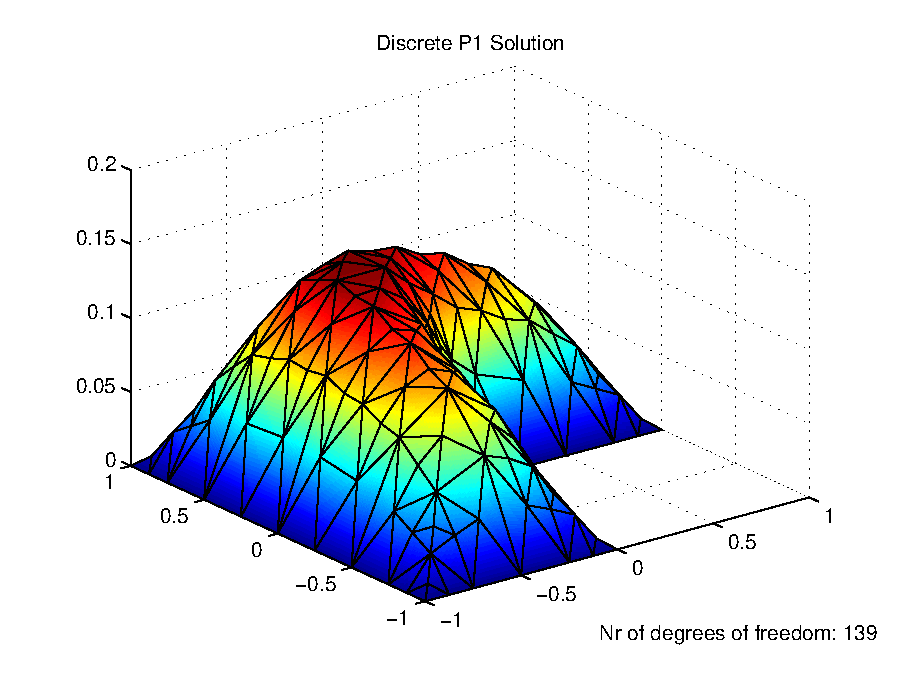
\includegraphics[width= 0.49\textwidth]{images/sect_QuickStart_LShapeU1}
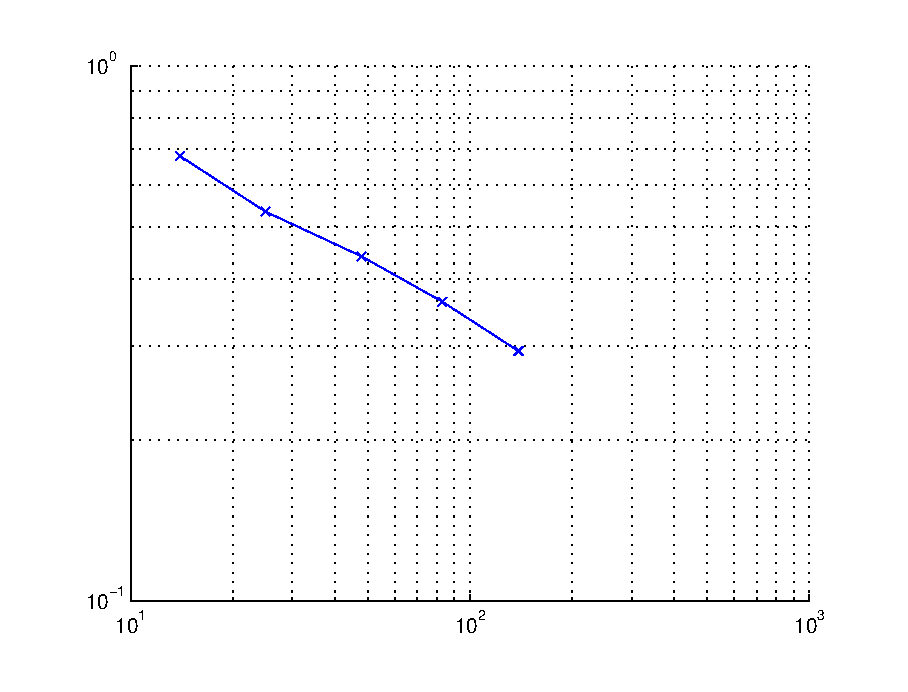
\includegraphics[width= 0.49\textwidth]{images/sect_QuickStart_LShapeE1}\\
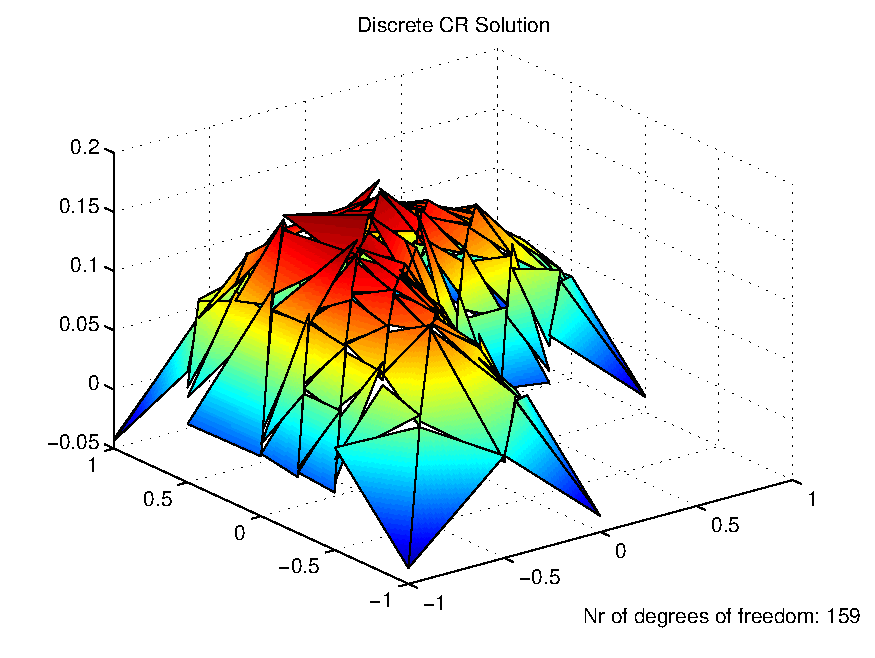
\includegraphics[width= 0.49\textwidth]{images/sect_QuickStart_LShapeU2}
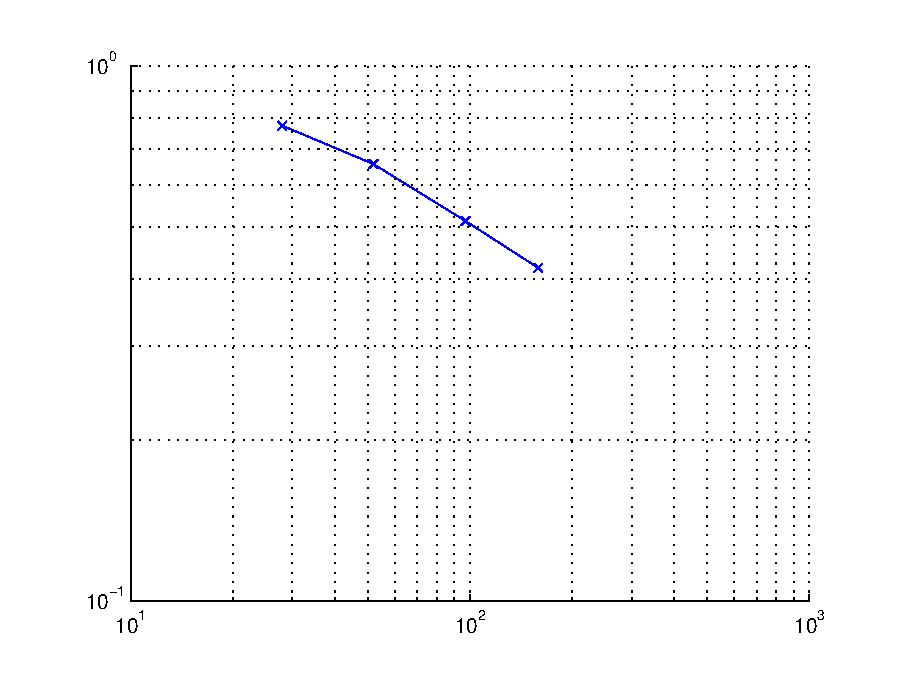
\includegraphics[width= 0.49\textwidth]{images/sect_QuickStart_LShapeE2}
\caption{Plots obtained from the \code{gettingStarted.m} script for \code{pdeSolver = 'P1'} on top and \code{pdeSolver = 'CR'} below.}\label{sect:Quickstart.fig.plots.gettingStarted}
\end{figure}

\clearpage

\subsection{Problem Definition}
\label{sect:QuickStart:ProblemDefinition}

This Subsection will try to explain the problem definition files. To make this more practical we will consider our elliptic example from Subsection~\ref{sect:QuickStart:gettingStarted}.\medskip\\
The actual problem definition looks as follows in Figure~\ref{sect:QuickStart.fig.problemDefinition}
\begin{figure}[ht!]

\begin{pcode}
function p = <name>(p)

p.problem.geom = <shape>;
p.problem.f = @<f>;
p.problem.g = @<g>;
p.problem.u_D = @<u_D>;
p.problem.kappa = @<kappa>;
p.problem.lambda = @<lambda>;
p.problem.mu = @<mu>;
\end{pcode}
\caption{}\label{sect:QuickStart.fig.problemDefinition}
\end{figure}

\noindent In the following table we will explain this code. \code{<f>}, \code{<g>}, \code{<u\_D>}, \code{<kappa>}, \code{<lambda>}, \code{<mu>} are functions that represent the corresponding functions of the problem. In general these have the following form:
\verb"function z = <name>(x,y,p)", where (\code{x},\code{y}) are the coordinates for all nodes (here supposed to be $N$), and \code{p} is the structure.\medskip

\begin{tabular}{p{0.2\textwidth}p{0.7\textwidth}}
\textit{} & Description\\\hline\\[-1ex]
\code{<name>}   & Any function name valid in MATLAB (should describes the problem definition).\\
\code{<shape>}  & This is the name of the folder that contains the data for a geometry.
                  Those folders have to be located at \path{.\problems\geometries\}.
                  For more information about what defines a geometry see Section~\ref{sect:DataStructures}\\
\code{<f>}      & Returns a vector with function values of $f$ of length $N$ calculated at $(x,y)$.\\
\code{<g>}      & Returns a vector of length $n$, where $n$ is the number of points
                  $(x,y)$ passed.\\
\code{<u\_D>}   & Returns a vector of length $n$, where $n$ is the number of points $(x,y)$ passed.\\
\code{<kappa>}  & Returns a $(2\times 2\times N)$ matrix, where the entry $(:,:,i)$ is the value of
                  $\kappa$ at node $i$, i.e., $\kappa(x_i,y_i) = z(:,:,i)$.\\
\code{<lambda>} & Returns a $(2\times N)$ matrix, where the entry $(:,i)$ is the value of
                  $\lambda$ at node $i$, i.e., $\lambda(x_i,y_i) = z(:,i)$.\\
\code{<mu>}     & Returns a vector of length $N$ that contains the function values of $\mu$ for every
                  node $(x_i,y_i)$.\\
\end{tabular}

\bigskip
\noindent Figure~\ref{sect:Quickstart.fig.code:problem} displays the full problem definition for an elliptic problem as in Section~\ref{sect:QuickStart:gettingStarted}.

\begin{figure}[hb!]
\inputcode{../problems/elliptic/Elliptic_Lshape.m}
\caption{Content of \code{Elliptic\_Lshape.m}}\label{sect:Quickstart.fig.code:problem}
\end{figure}
\clearpage

\subsection{How to Implement a Problem}
\label{sect:QuickStart:howToOwnProblem}

In this subsection we describe how one can easily use the implemented methods in the \FFW to solve problems with ones own data. To explain how to change the data we look at the example of a elliptic PDE of the form

\begin{align*}
- \ddiv (\kappa \,\grad u) + \lambda \,\grad u + \mu \, u &= f &&\text{in } \Omega,\\
u &= u_D &&\text{on } \Gamma,\\
\frac{\partial u}{\partial n} &= g &&\text{on } \partial\Omega \setminus \Gamma,
\end{align*}

In general there are two ways to implement a problem. If one wants to test a method of the \FFW with an exact analytic solution and an elliptic operator like the one above, one can use the template \path{Elliptic_Exact_Template.m} in \path{.\problems\elliptic}. One has to copy the file and rename the copy. In the copy of the template one can change the symbolic expressions for $u$, $\kappa$, $\lambda$ and $\mu$ then the right hand side $f$ is calculated automatically such that $u$ is the solution of the PDE. The relevant part of the template \path{.\Elliptic_Exact_Template.m} looks as follows:

\begin{pcode}
% Specification of exact solution and differential Operator
u = sin(x^3)*cos(y^pi)+x^8-y^9+x^6*y^10;
lambda = [0, 0];
mu = 0;
kappa = [1 0; 0 1];
\end{pcode}

If one wants to solve a given problem, one uses the template \path{Elliptic_Template.m} in \path{.\problems\elliptic}. In the renamed copy one has to change the function definitions of the data. The relevant part of the template \path{Elliptic_Template.m} looks as follows:

\begin{pcode}
%%%%%%%%%%%%%%%%%%%%%%%%%%%%%%%%%%%%%%%%%%%%%%%%%%%%%%%%%%%%%%%%%%%%%%%

% Volume force
function z = f(x,y,p)
z = ones(length(x),1);

%%%%%%%%%%%%%%%%%%%%%%%%%%%%%%%%%%%%%%%%%%%%%%%%%%%%%%%%%%%%%%%%%%%%%%%

% Dirichlet boundary values
function z = u_D(x,y,p)
z = zeros(length(x),1);

%%%%%%%%%%%%%%%%%%%%%%%%%%%%%%%%%%%%%%%%%%%%%%%%%%%%%%%%%%%%%%%%%%%%%%%
% Neumann boundary values
function z = g(x,y,n,p)
z = zeros(length(x),1);

%%%%%%%%%%%%%%%%%%%%%%%%%%%%%%%%%%%%%%%%%%%%%%%%%%%%%%%%%%%%%%%%%%%%%%%

% elliptic PDE coefficent kappa ( div(kappa*grad_u) )
function z = kappa(x,y,p)
nrPoints = length(x);
z = zeros(2,2,nrPoints);
for curPoint = 1:nrPoints
    z(:,:,curPoint) = [1 0;
                      0 1];
end
%%%%%%%%%%%%%%%%%%%%%%%%%%%%%%%%%%%%%%%%%%%%%%%%%%%%%%%%%%%%%%%%%%%%%%%

% elliptic PDE coefficent lambda ( lambda*grad_u )
function z = lambda(x,y,p)
nrPoints = length(x);
z = zeros(nrPoints,2);
for curPoint = 1:nrPoints
    z(curPoint,:) = [0 , 0];
end

%%%%%%%%%%%%%%%%%%%%%%%%%%%%%%%%%%%%%%%%%%%%%%%%%%%%%%%%%%%%%%%%%%%%%%%

% elliptic PDE coefficent mu ( mu*u )
function z = mu(x,y,p)
z = zeros(length(x),1);

%%%%%%%%%%%%%%%%%%%%%%%%%%%%%%%%%%%%%%%%%%%%%%%%%%%%%%%%%%%%%%%%%%%%%%%
\end{pcode}

If one wants to change the geometry of $\Omega$, one can use one of the implemented geometries in \path{.\problems\geometries} by changing the geometry in the PDE definition in the copy of the template file to the name of the folder containing the data.
% PDE definition
p.problem.geom = 'Lshape';

To use a new geometry one has to create a new folder in \path{.\problems\geometries} which contains the data files \path{<geometry name>_n4e.dat}, \path{<geometry name>_c4n.dat}, \path{<geometry name>_Db.dat} and \path{<geometry name>_Nb.dat}. Here \path{<geometry name>} is the name of the created folder. To see how the geometry data must be structured see Section~\ref{sect:DataStructures} and the already existing folders.

In \path{start_elliptic.m} the new Problem is chosen by
\begin{pcode}
problem = '<name of file>'
\end{pcode}
where \path{<name of file>} is the name of the copy from the template.






\section{Flow Chart}
\label{sect:FlowChart}

\noindent This Section is devoted to the structure of the \FFW and illustrates to flow of the framework. In Figure~\ref{sect:FlowChart.fig.FFW-flowchart} one can see this structure in a flow chart.

\begin{figure}[ht!]
\footnotesize
\begin{equation*}
\xymatrix@-1eM{
    *+<2ex>[F]{ \phantom{I}\text{script}\phantom{I} }           \ar@{=>}[r]
&   *+<2ex>[F]{ \phantom{I}\code{initFFW}\phantom{I} }          \ar@{=>}[r]\ar@{->}[d]
&   *+<2ex>[F]{ \phantom{I}\code{computeSolution}\phantom{I} }  \ar@{=>}[r] \ar@{->}[d]^{\text{loop}}
&   *+<2ex>[F]{ \phantom{I}\text{output}\phantom{I} }
\\
& *+[F-:<3pt>]{ \code{problemType-init}} \ar@{->}[d]   &  *+[F-:<3pt>]{ \code{afem} }            \ar@{->}[d]
\\
&*+[F-:<3pt>]{ \code{pdeSolver-init}} &  *+[F-:<3pt>]{ \code{mark} }            \ar@{->}[d]
\\
&& *+[F-:<3pt>]{ \code{refine} }          \ar@{->}[d]
\\
&& *+[F-:<3pt>]{ \code{enumerate} }       \ar@{.>}[r] \ar@{->}[d]
&   *+[F-:<3pt>]{ \code{genericEnumerate} }
\\
&& *+[F-:<3pt>]{ \code{createLinSys} }    \ar@{->}[d]
\\
&& *+[F-:<3pt>]{ \code{solve} }           \ar@{->}[d]
\\
&& *+[F-:<3pt>]{ \code{postProc} }        \ar@{->}[d]
\\
&& *+[F-:<3pt>]{ \code{estimate} }        \ar@{->}'l[u] '[uu] [uu]
}
\end{equation*}
\normalsize \caption{Flow chart of the \FFW.}\label{sect:FlowChart.fig.FFW-flowchart}
\end{figure}

\begin{longtable}{p{0.25\textwidth}p{0.65\textwidth}}
function name & description\\\hline\\[-1ex]

\text{script} & control script, examples are \code{start\-Scalar}
                and \code{start\-Elasticity}\\
\code{initFFW} & sets paths, loads default parameters,
                 sets supplied parameters and loads problem definition and geometry\\
\code{problemType-init} & creates method specific
             function handles, e.g. a function handle to evaluate
             the discrete solution\\
\code{pdeSolver-init} & creates finite element space specific
             function handles, e.g. a function handle to eval the basis functions\\
\code{computeSolution} & calls \code{afem} as long as some abort criteria defined
                         in the configuration file, e.g., \code{maxNrDoF},
                         is not fulfilled and supplies method type specific
                         function handles, e.g. a function to evaluate
                         the energy error\\
\code{afem} & calls \code{mark}, \code{refine}, \code{enumerate},
              \code{createLinSys}, \code{solve}, \code{postProc} and
              \code{estimate}\\
\code{mark} & marks edges and triangles for refinement based on an error
              estimator (\code{bulk}, \code{max}) with additional edges to
              maintain shape regularity, or marks all edges (\code{uniform})\\
\code{refine} & refines the list of edges supplied by mark\\
\code{enumerate} & calls \code{genericEnumerate} and computes method
                   specific data structures from the triangulation,
                   e.g., the number of degrees of freedom\\
\code{genericEnumerate} & creates useful data structures from the current
                          triangulation, e.g., normals, tangents, areas\\
\code{createLinSys} & assembles the global linear system of equations $Ax=b$\\
\code{solve} & computes $x$\\
\code{postProc} & post processing of the solution, e.g., separating Lagrange
                  multipliers form the discrete solution\\
\code{estimate} & locally estimates the error based on the discrete solution\\
\text{output} & user specific data evaluation
\end{longtable}

\section{Implemented Problems}
\label{sect:ImplementedProblems}
In this section we give an overview about the implemented problems. At first we present the strong and weak formulation for the full elliptic PDE and for a problem in elasticity. There we define the spaces for the conforming and non-conforming discretizations. Additionally we take a look on the mixed formulation with the corresponding spaces. In the \FFW there are several problems and geometries already defined. In ./problems/geometries you will find the definition of the geometries, e.g. L-shape or Square, and in ./problems/elliptic (./problems/elasticity) we give some examples for a problem definition for an elliptic (elasticity) problem.

\subsection{FEM for Elliptic PDEs}
We consider the following elliptic PDE

\begin{align}
\label{sect:FEMForEllipticProblems.eq.strongForm}
  -\ddiv(\kappa\cdot\nabla u) + \lambda\cdot\nabla u + \mu u &= f &\text{in } \Omega, \\
  u &= u_D &\text{ on } \Gamma_D, \\
  \nabla u\cdot\nu &= g &\text{ on } \Gamma_N
\end{align}

with $u_D\in~H^1(\Omega;\R)$, $f\in~L^2(\Omega;\R)$, $g\in~L^2(\Gamma_N;\R)$, $\kappa\in~L^\infty(\Omega;\R^{2\times 2})$, $\lambda\in~L^{\infty}(\Omega,\R^2)$ and $\mu\in~L^\infty(\Omega,\R)$. 

\bigskip

\noindent The weak form of \eqref{sect:FEMForEllipticProblems.eq.strongForm} reads: For all $v\in V$ seek $u\in V$ such that
\begin{align}
\label{sect:FEMForEllipticProblems.eq.weakForm}
	\int_\Omega \left( \nabla u\cdot(\kappa\cdot\nabla v) + \lambda\cdot\nabla u\,v + \mu u\,v\right )\,dx = \int_\Omega f\,v\,dx + \int_{\Gamma_N} g\,v\,ds_x.
\end{align}

\bigskip

We have implemented a conforming disretization of \eqref{sect:FEMForEllipticProblems.eq.weakForm} with $V$ being the space of piecewise affine and globally continuous functions and a nonconforming method with $V$ consisting the piecewise affine functions which are continuous at the midpoints of the edges $\mathcal{E}$ of a triangulation $\mathcal{T}$.

\bigskip

The mixed formulation of \eqref{sect:FEMForEllipticProblems.eq.strongForm} reads

\begin{align}
\label{sect:FEMForEllipticProblems.eq.mixedStrongForm}
  -\ddiv\sigma + \lambda\cdot(\kappa^{-1}\cdot\sigma) + \mu u &= f &\text{in } \Omega, \\
  \sigma &= \kappa\cdot\nabla u &\text{in } \Omega,\\
  u &= u_D &\text{ on } \Gamma_D, \\
  (\kappa^{-1}\cdot\sigma)\cdot\nu &= g &\text{ on } \Gamma_N
\end{align}

with the corresponding weak form

\begin{align}
\label{sect:FEMForEllipticProblems.eq.mixedWeakForm}
  \int_\Omega \left( -\ddiv\sigma\,v + \lambda\cdot(\kappa^{-1}\cdot\sigma)\,v + \mu u\,v\right)\,dx &= \int_\Omega f\,v\,dx &\text{for all } v\in V, \\
  \int_\Omega \left((\kappa^{-1}\cdot\sigma)\cdot\tau + \ddiv\tau\, u\right)\,dx &= \int_{\Gamma_D} u_D(\tau\cdot\nu)\,ds_x &\text{for all } \tau\in\Sigma.
\end{align}

\bigskip

We have implemented the mixed Raviart-Thomas finite element $RT_0\times P_0$ where $\Sigma$ consists of piecewise affine functions where continuity is enforced only in normal direction $\nu$ across each edge of a triangulation $\mathcal{T}$. The space $V$ consists of piecewise constant functions.

\bigskip
\subsection{FEM for Elasticity}

\noindent In theory of linear elasticity one is interested in the solution of the following system of elliptic PDE's:
\begin{align}\label{elasticity strong form}
-\ddiv\, \C\,\varepsilon(u)&=f &&\text{in }\Omega,\nonumber\\
u&=u_D &&\text{on }\Gamma_D,\\
(\C\,\varepsilon(u))\cdot \nu&=g &&\text{on }\Gamma_N,\nonumber
\end{align}
with $u_D\in H^1(\Omega;\R^2)$, $f\in L^2(\Omega;\R^2)$, $g\in L^2(\Gamma_N;\R^2)$. Here and throughout, $\varepsilon(v)=\frac{1}{2}(\grad v+(\grad v)^T)$ denotes the linearized Green strain tensor, $\C$ is the reduced symmetric fourth order bounded and positive definite elasticity tensor defined by the Lam\'e parameters $\lambda$ and $\mu$. In Voigt notation the tensor $\C$ and its inverse is given through
\begin{equation*}
\C:=\begin{pmatrix}
2\mu+\lambda & \lambda       & 0\\
\lambda      & 2\mu+\lambda  & 0\\
0            & 0             & \mu
\end{pmatrix} \quad\text{and}\quad
\Cinv:=\begin{pmatrix}
\frac{\lambda+2 \mu}{4\mu(\lambda+\mu)} & \frac{-\lambda}{4\mu(\lambda+\mu)}            & 0\\
\frac{-\lambda}{4\mu(\lambda+\mu)}          & \frac{\lambda+2 \mu}{4\mu(\lambda+\mu)} & 0\\
0 & 0 & \frac{1}{\mu}
\end{pmatrix}.
\end{equation*}

\noindent There are several formulations of the problem \eqref{elasticity strong form} depending on the focus of interest. For instant, \eqref{elasticity strong form} is a displacement based formulation. Here, one computes an approximation of the displacement $u$ and afterwards the discrete solution $u_h$ is post-processed to get the discrete strain and stress of the problem. In other formulations strain or stress are computed directly. The \FFW offers a displacement-based and a stress-displacement-based formulation. Both can be found in \cite{Bra}.

\bigskip

\noindent Similar to the elliptic problems, there are conforming and nonconforming FE-methods which one can choose to solve \eqref{elasticity strong form}. At first, the weak formulation is given: Seek $u\in V$ such that
\begin{equation}\label{elasticity weak form}
\int_{\Omega} \varepsilon(u):\C\varepsilon(v) \, dx = \int_{\Omega}
f \cdot v \, dx + \int_{\Gamma_N} g\cdot v \, ds_x \quad\text{for
all } v \in V.
\end{equation}

\noindent The conforming $P_1-P_1$ FE-method approximates the displacement $u\in H^1(\Omega)^2$ in each component with the linear ansatz space $P_1$. Since this kind of approximations does not work for incompressible materials like rubber or water, the so-called locking effect, there is also a nonconforming method available. The Kouhia-Stenberg element ($P_1-CR$) approximates the first component of $u$ with the globally continuous piecewise linear ansatz-space ($P_1$) and the second one with the Crouzeix-Raviart ansatz-space ($CR$). The Kouhia-Stenberg element is able to handle also incompressible materials. Details can be found in \cite{Bra,KoSt}. Problems will arise in the condition number of the energy matrix for incompressible materials. To get rid of it one has to change the problem formulation. A stress-displacement formulation which results in a mixed scheme handles then both problems: the locking effect and the dependence of the condition number for incompressible materials. This formulation and the FE-spaces we will describe as next.

\bigskip

%\noindent If the main interest is on an accurate stress or flux approximation and some strict equilibration
%condition rather than the displacement, it might be advantageous to consider an operator split: Instead of
%one partial differential equation of order $2m$ one considers two equations of order $m$.
%To be more precise, given one equation in an abstract form $\mathcal{L}u = G$ with some differential
%operator $\mathcal{L} = \mathcal{A}\mathcal{B}$ composed of $\mathcal{A}$ and $\mathcal{B}$, define $p := \mathcal{B}u$ and solve the two equations
%$\mathcal{A}p = G$ and $\mathcal{B}u = p$.\smallskip\\
%\noindent
%The mixed form of \eqref{elasticity strong form} reads:

\noindent The stress-displacement formulation of \eqref{elasticity strong form} is given through: Seek $(\sigma,u)\in\Sigma\times V$ such that
\begin{align}\label{elasticity mixed strong form}
		-\ddiv\, \sigma&=f&  &\text{ and }& \sigma&=\C\,\varepsilon(u)&\text{  in }\Omega,\\
		u&=u_D\text{ on }\Gamma_D& &\text{ and }& \sigma \nu&=g \text{ on }\Gamma_N.\nonumber
\end{align}
Then, the corresponding weak form reads
\begin{align*}
\int_{\Omega} \sigma:\C^{-1}\tau \, dx + \int_{\Omega} u\cdot\ddiv\,
\tau \,dx
&= \int_{\Gamma_D} u_D\cdot (\tau \,\nu) \, ds_x &&\text{for all } \tau \in \Sigma,\\
\int_{\Omega} v\cdot\ddiv\, \sigma\,dx &= - \int_{\Omega} f \cdot v
\, dx &&\text{for all } v \in V.
\end{align*}

\noindent One way to handle \eqref{elasticity mixed strong form} is the Peers-element which is described in \cite{CCDo}. The problem with that element is symmetry of the stress $\sigma$. This is only enforced weakly with a side constraint. In the \FFW we have implemented another mixed finite element based on the work of Arnold and Winther \cite{ArWi}. They have introduced a mixed finite element of problem \eqref{elasticity mixed strong form} which is locking-free (with a condition number which is independent of the current material) and the discrete stress $\sigma_h$ is symmetric in a natural way. Details on the implementation can be found in \cite{CCGuReTh}.

\bigskip
\subsection{Predefined Problem Definitions}
\label{sect:ImplementedProblems_ProblemDefinition}

\noindent There are various problem definitions for elliptic PDEs and for linear elasticity already defined, for which we give an overview in the following.

\medskip

\noindent All problem definitions contain functions for the coefficients $\kappa$, $\lambda$, $\mu$, the external load $f$, and the boundary $u_D$ and $g$. Some of the problem-definition-filenames contain a suffix \path{_exact}. Here a function $u_{\text{exact}}$ which represents the exact solution is given and the data-functions $f$, $u_D$ and $g$ are computed automatically. With those problem definitions it is possible to compute the exact errors, e.g. energy error between $u_h$ and $u_{\text{exact}}$. Problem definitions for elasticity additionally contain standard parameters for the material parameter $\nu$ and $E$.

\bigskip

\noindent If you want to create your own problem definition, create an \code{.m}-file named \path{Elliptic_<problemName>} in \path{.\problems\elliptic} or \path{Elasticity_<problemName>} in (\path{.\problems\elasticity}), which contains all necessary information. For details concerning the structure of the problem definition, see Section \ref{sect:QuickStart}.

\bigskip

\subsubsection{Predefined Problem Definitions for Elliptic PDEs}$ $\\

\noindent\emph{Elliptic\_Lshape}

\smallskip

\noindent Model example $-\Delta u = 1$, $u_D=0$ and $g=0$ on an L-shaped domain.

\bigskip

\noindent\emph{Elliptic\_Lshape\_exact}

\smallskip

\noindent The exact solution $u(r,\phi)=r^{2/3}\sin(2/3\phi)$ in polar coordinates on an L-shaped domain with Neumann boundary is given. The corresponding right hand side $f$ is zero and induced boundary data. The coefficients of the elliptic PDE correspond to the Laplacian operator.
\bigskip

\noindent\emph{Elliptic\_Square}\smallskip\\
Model example $-\Delta u = 1$, $u_D=0$ and $g=0$ on a squared domain.
\bigskip

\noindent\emph{Elliptic\_Square\_exact}\smallskip\\
The exact solution $u(x,y) = x(1-x)\,y(1-y)$ as well as its gradient and the right-hand side $f$ are given with the PDE-coefficients $\kappa$, $\lambda$ and $\mu$ all zero, on a squared domain is given.
\bigskip

\noindent\emph{Elliptic\_SquareFullElliptic\_exact}\smallskip\\
The exact solution $u(x,y) = \sin(x^3)\cos(y^\pi)+x^8-y^9+x^6 y^{10}$ with the PDE-coefficients $\kappa$ being the identity, $\lambda = \left( \begin{smallmatrix} 5\sin(x+y)\\ 6\cos(x+y) \end{smallmatrix}\right)$ and $\mu=7$ on a squared domain is given. The symbolic toolbox of MATLAB computes all necessary information, i.e., $f$, $u_D$ and $g$.
\bigskip

\noindent\emph{Elliptic\_HexagonalSlit\_exact}\smallskip\\
The exact solution $u(r,\phi)=r^{1/4}\sin(1/4\phi)$ in polar coordinates with the load $f\equiv0$, the Dirichlet function $u_D=u|_{\Gamma_D}$, and coefficients belonging to the Laplacian are given on a slitted hexagon.
\bigskip

\noindent\emph{Elliptic\_Waterfall\_exact}\smallskip\\
The waterfall function $$u(x,y) = xy(1-x)(1-y) \arctan\left(k(\sqrt{(x-5/4)^2 + (y+1/4)^2}-1)\right)$$ is given. The parameter $k$ controls the slope of $u$. For $k\rightarrow\infty$ the slope of the function tends to infinity. This parameter is stored in the structure \code{p} at \code{p.PDE.k} and can be changed in the starting scripts. The domain is a square with homogeneous Dirichlet boundary. We look at the problem $-\Delta u = f$. The load $f$ is computed from $u$.
\bigskip

\noindent\emph{Elliptic\_Template}\smallskip\\
A predefined template for generating problem definitions. For given data $f, u_D$ and $g$ one can compute the corresponding discrete solution $u_h$.
\bigskip

\noindent\emph{Elliptic\_Template\_Exact}\smallskip\\
A predefined template for generating problem definitions. For a given function $u_{\text{exact}}(x,y)$ in cartesian coordinates and coefficients $\kappa,\lambda,\mu$, the symbolic toolbox of MATLAB computes all necessary information, i.e., $f$, $u_D$ and $g$.
\bigskip


\subsubsection{Predefined Problem Definitions for Elasticity}$ $\\

\noindent\emph{Elasticity\_Cooks}\smallskip\\
A tapered panel is clamped on one end and subjected to a surface load in
vertical direction on the opposite end with $f = 0$ and $g(x, y) = (0, 1000)$ if
$(x, y) \in  \Gamma_N$ with $x = 48$ and $g = 0$ on the remaining part of $\Gamma_N$, the Young modulo $E =
2900$, and the Possion ratio $\nu = 0.3$.
\bigskip


\noindent\emph{Elasticity\_Square\_exact}\smallskip\\
The unit square with the given function $u(x,y)=10^{-5}\left(\begin{smallmatrix} \cos((x+1)(y+1)^2) \\
\sin((x+1))\cos(y+1) \end{smallmatrix}\right)$. Young modulo and the Possion ratio are set to $E=10^5$ and $\nu = 0.3$.
\bigskip


\noindent\emph{Elasticity\_Square\_Neumann\_exact}\smallskip\\
Besides the geometry we have the same problem definition as in \emph{Elasticity\_Square}. The domain changes from \code{Square} to \code{SquareNeumann}.
\bigskip


\noindent\emph{Elasticity\_Lshape\_exact}\smallskip\\
Using polar coordinates $(r, \theta)$, $-\pi < \theta \leq \pi$ $u$ with radial component $u_r,u_\theta$ reads
$$
u_{r}(r,\theta) = \frac{r^{\alpha}}{2\mu}
    (-(\alpha+1)\cos((\alpha+1)\theta)+
           \nonumber     (C_{2}-
    (\alpha+1))C_{1}\cos((\alpha-1)\theta)),
$$
and
$$ u_{\theta}(r,\theta) = \frac{r^{\alpha}}{2\mu}
    ((\alpha+1)\sin((\alpha+1)\theta)+
          \nonumber     (C_{2}+\alpha-1)C_{1}\sin((\alpha-1)\theta)).
$$
The parameters are
$C_{1}=-\cos((\alpha+1)\omega)/\cos((\alpha-1)\omega)$, $C_{2} = 2(\lambda+2\mu)/(\lambda+\mu)$ where $\alpha = 0.54448...$ is the positive solution of  $\alpha \sin 2\omega + \sin 2\omega\alpha = 0$ for $ \omega= 3 \pi /4$; the Young modulus is $E=10^5$, Poisson ratio $\nu = 0.3$, and the volume force $f\equiv 0$.
\bigskip


\noindent\emph{Elasticity\_Template}\smallskip\\
A predefined template for generating problem definitions. For given data $f,u_D$ and $g$ and coefficients $\kappa,\lambda,\mu$ one can compute the corresponding discrete solution $u_h$.
\bigskip


\noindent\emph{Elasticity\_Exact\_Template}\smallskip\\
A predefined template for generating problem definitions. For a given function $u_{\text{exact}}(x,y)$ in cartesian coordinates, the symbolic toolbox of MATLAB computes all necessary information, i.e., $f$, $u_D$ and $g$. 
\bigskip
\subsection{Geometries}
\label{sect:ImplementedProblems_Geometries}

In the following we give an overview about the geometries which are already available.\medskip\\
To add a new geometry create a new directory \code{<newGeometry>} in \path{.\problems\geometries\}. There you have to define the coordinates of the geometry in \path{<newGeometry>_c4n.dat}. The nodes for each element, e.g. triangle, have to be defined in \path{<newGeometry>_n4e.dat}. The Dirichlet- and Neumann-part of the domain boundary is specified in \path{<newGeometry>_Db.dat} and \path{<newGeometry>_Nb.dat} respectively.
\bigskip

\newpage
\noindent\emph{Triangle}\smallskip\\
\begin{minipage}{0.14\textwidth}
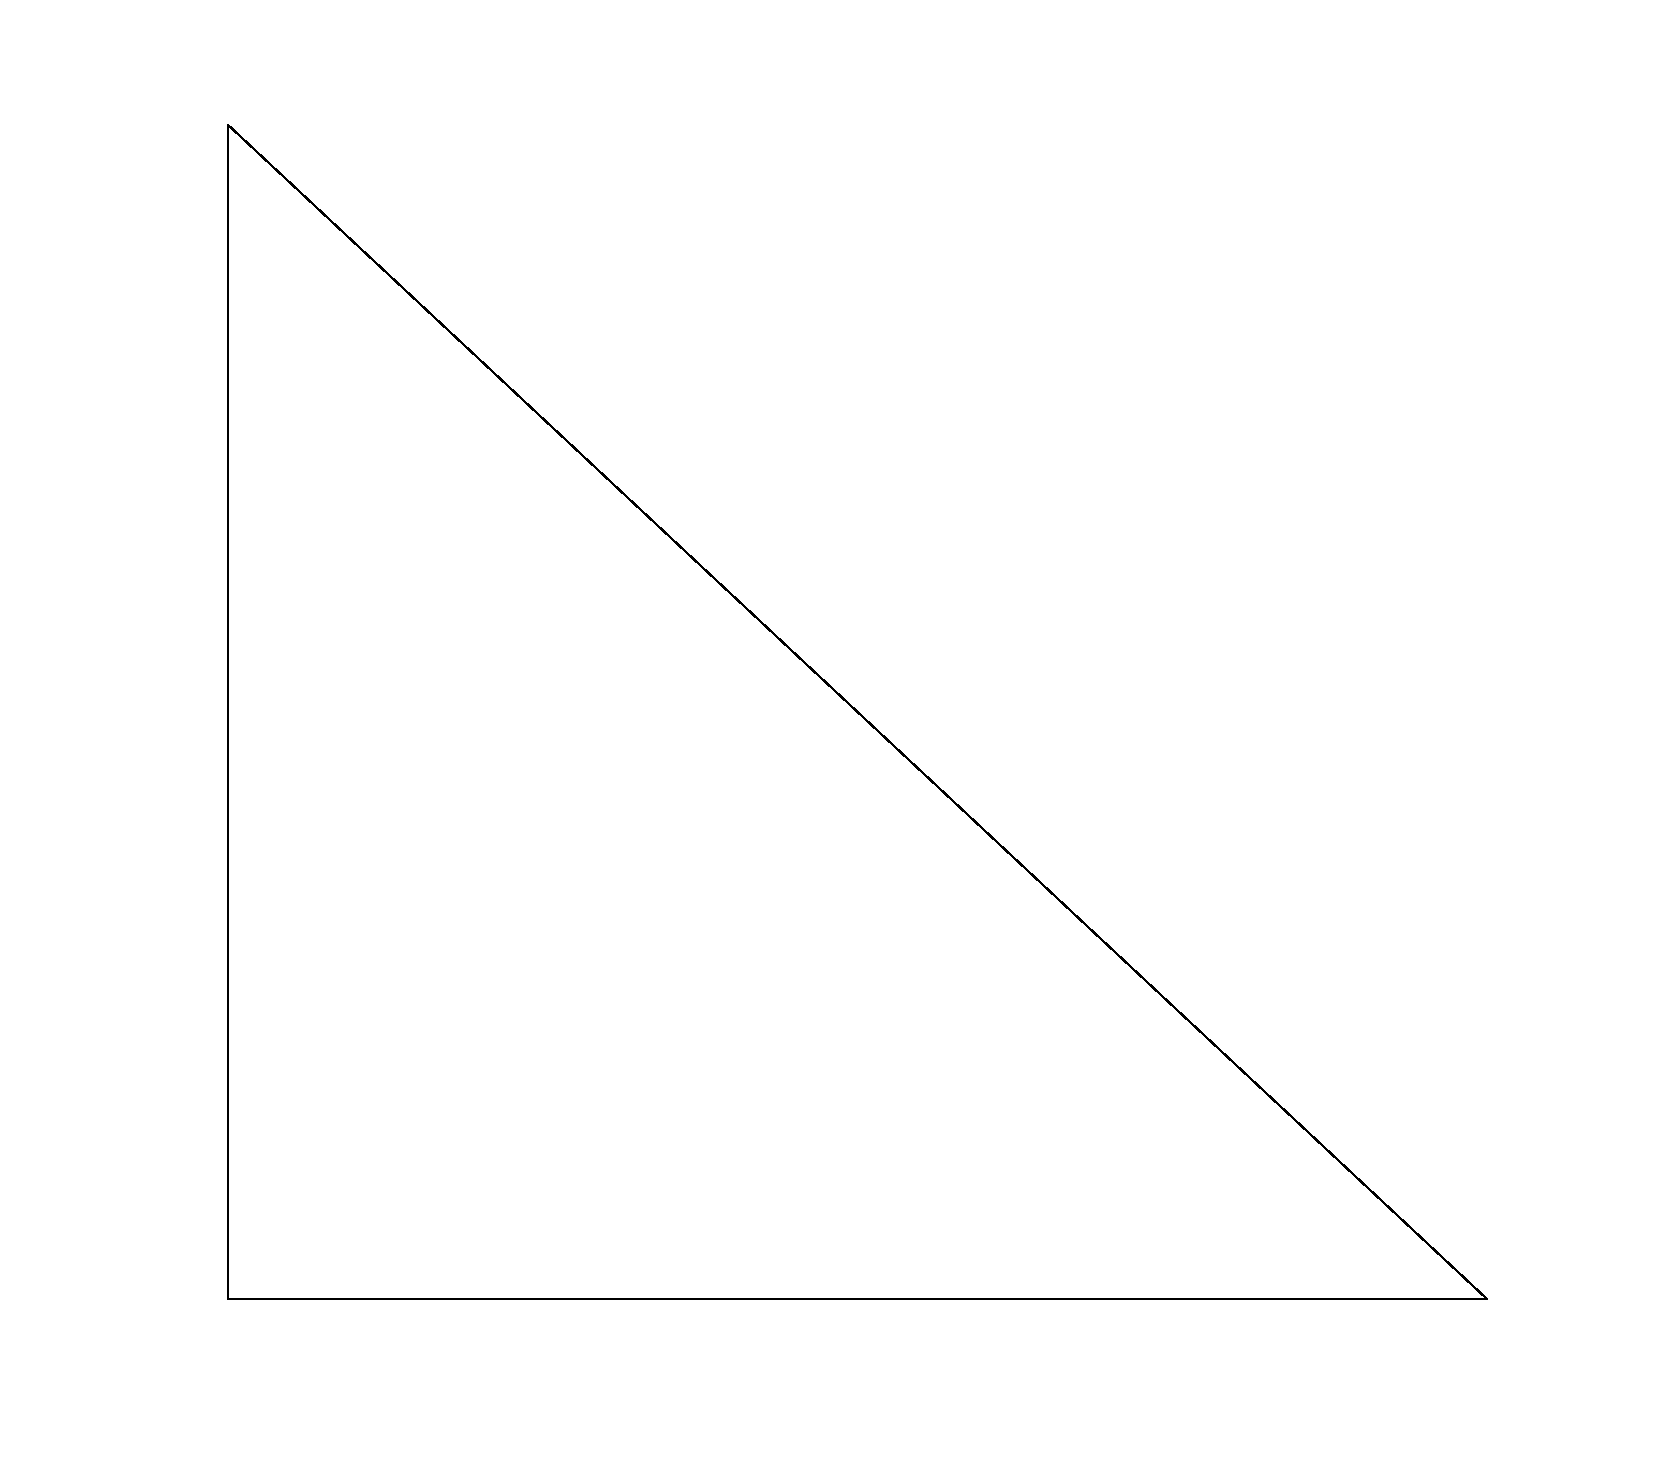
\includegraphics[width=0.9\textwidth]{images/sect_ImplementedProblems_Triangle}
\end{minipage}
\begin{minipage}{0.85\textwidth}
The reference triangle $\Omega=\conv\{(0,0),(1,0),(0,1)\}$ with pure Dirichlet-boundary.
\end{minipage}
\bigskip

\noindent\emph{Square}\smallskip\\
\begin{minipage}{0.14\textwidth}
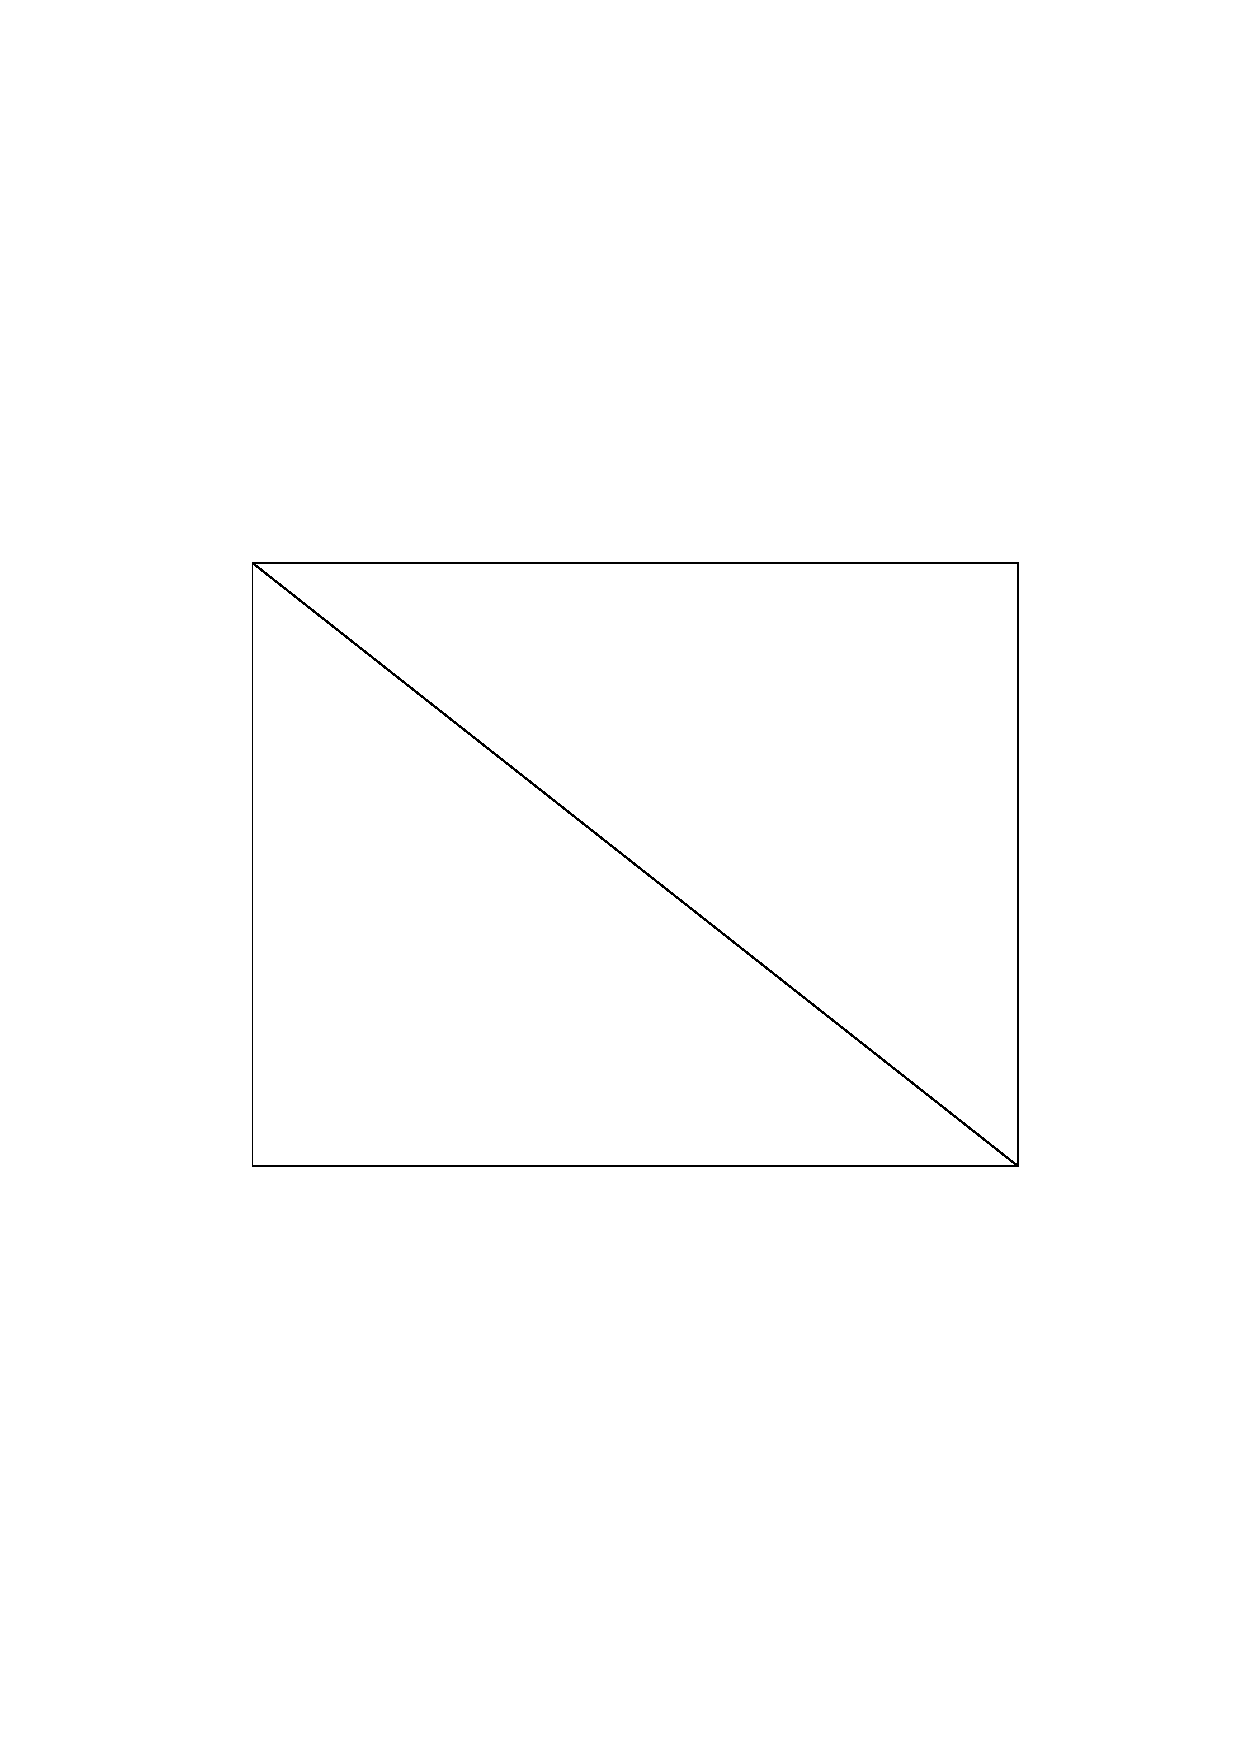
\includegraphics[width=0.9\textwidth]{images/sect_ImplementedProblems_Square.pdf}
\end{minipage}
\begin{minipage}{0.85\textwidth}
The unit square $\Omega=[0,1]^2$ with pure Dirichlet-boundary.
\end{minipage}
\bigskip

\noindent\emph{SquareNeumann}\smallskip\\
\begin{minipage}{0.14\textwidth}
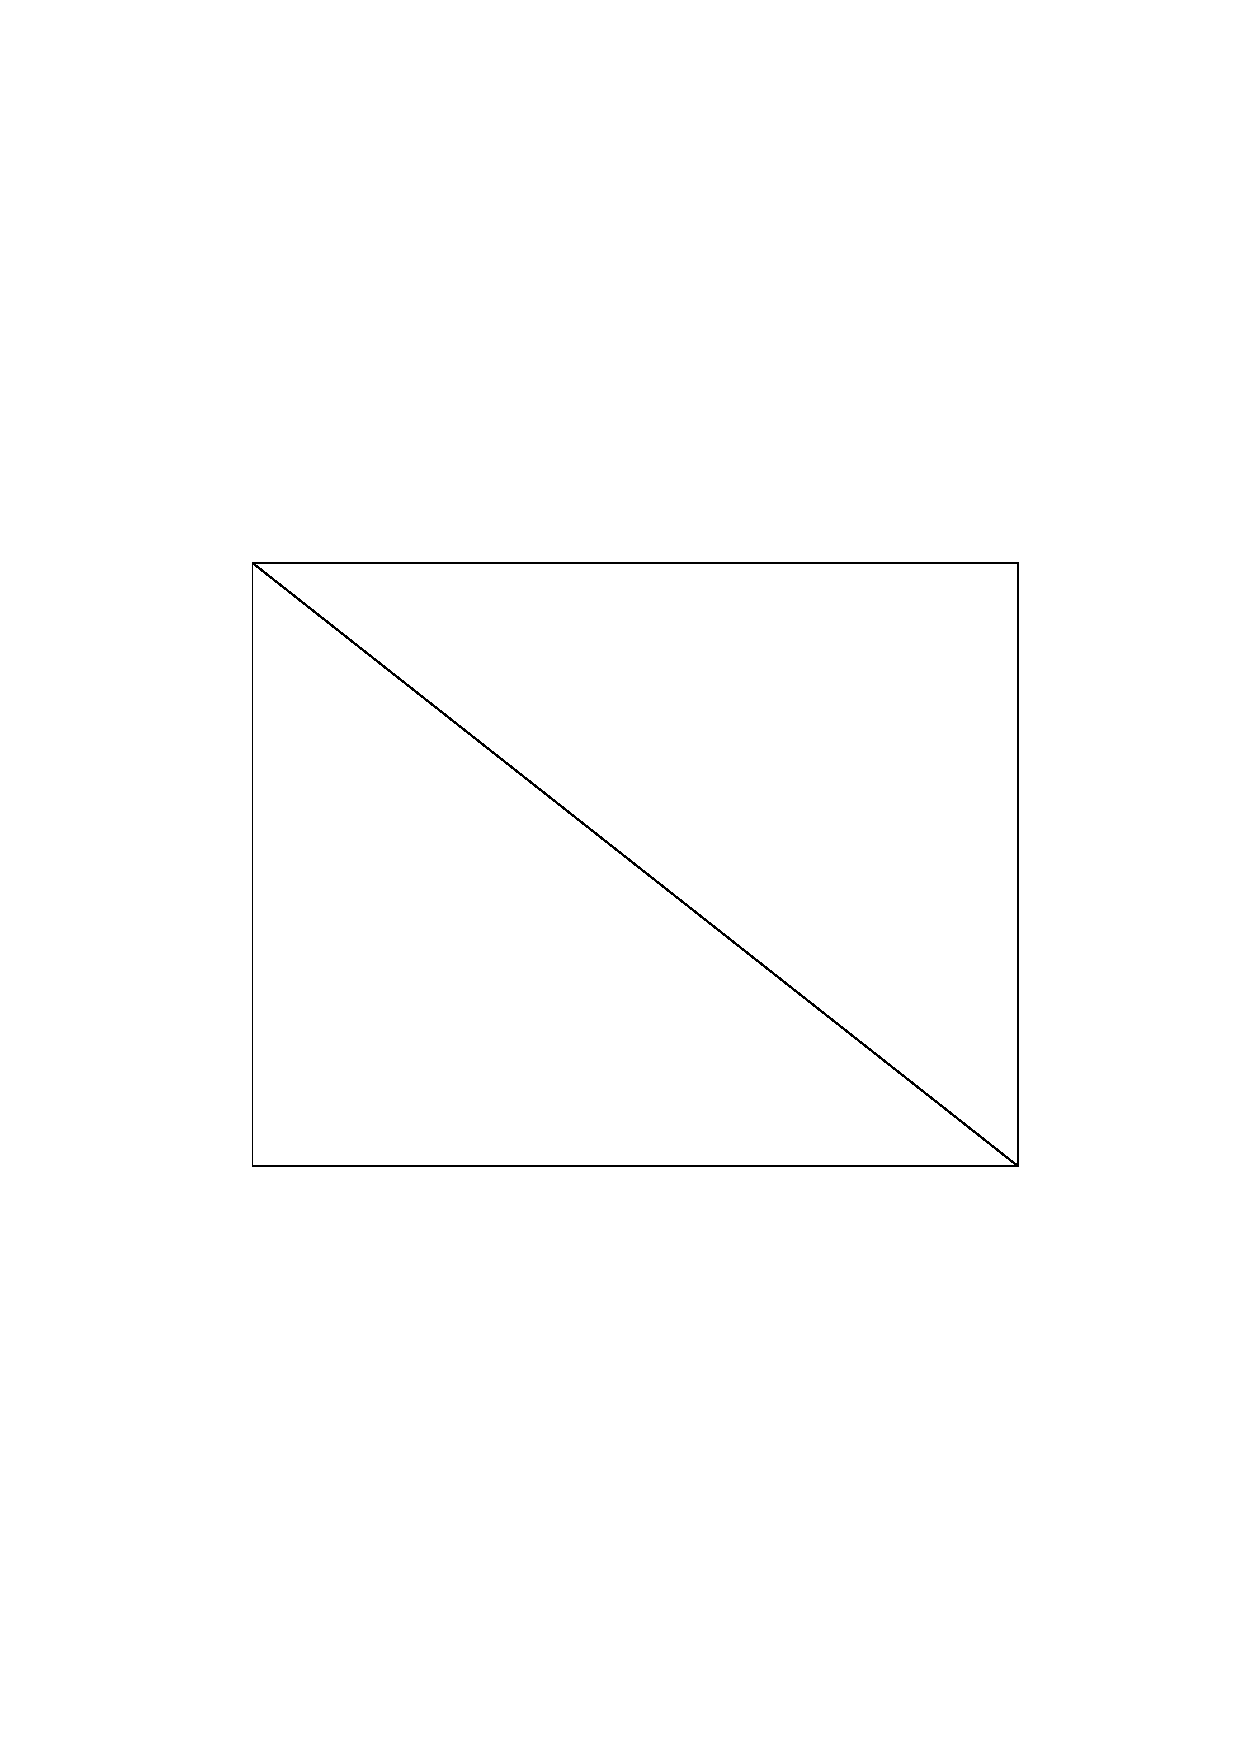
\includegraphics[width=0.9\textwidth]{images/sect_ImplementedProblems_Square.pdf}
\end{minipage}
\begin{minipage}{0.85\textwidth}
The unit square with Neumann boundary $\Gamma_N=\conv\{(1,0),(1,1)\}$.
\end{minipage}
\bigskip

\noindent\emph{Lshape}\smallskip\\
\begin{minipage}{0.14\textwidth}
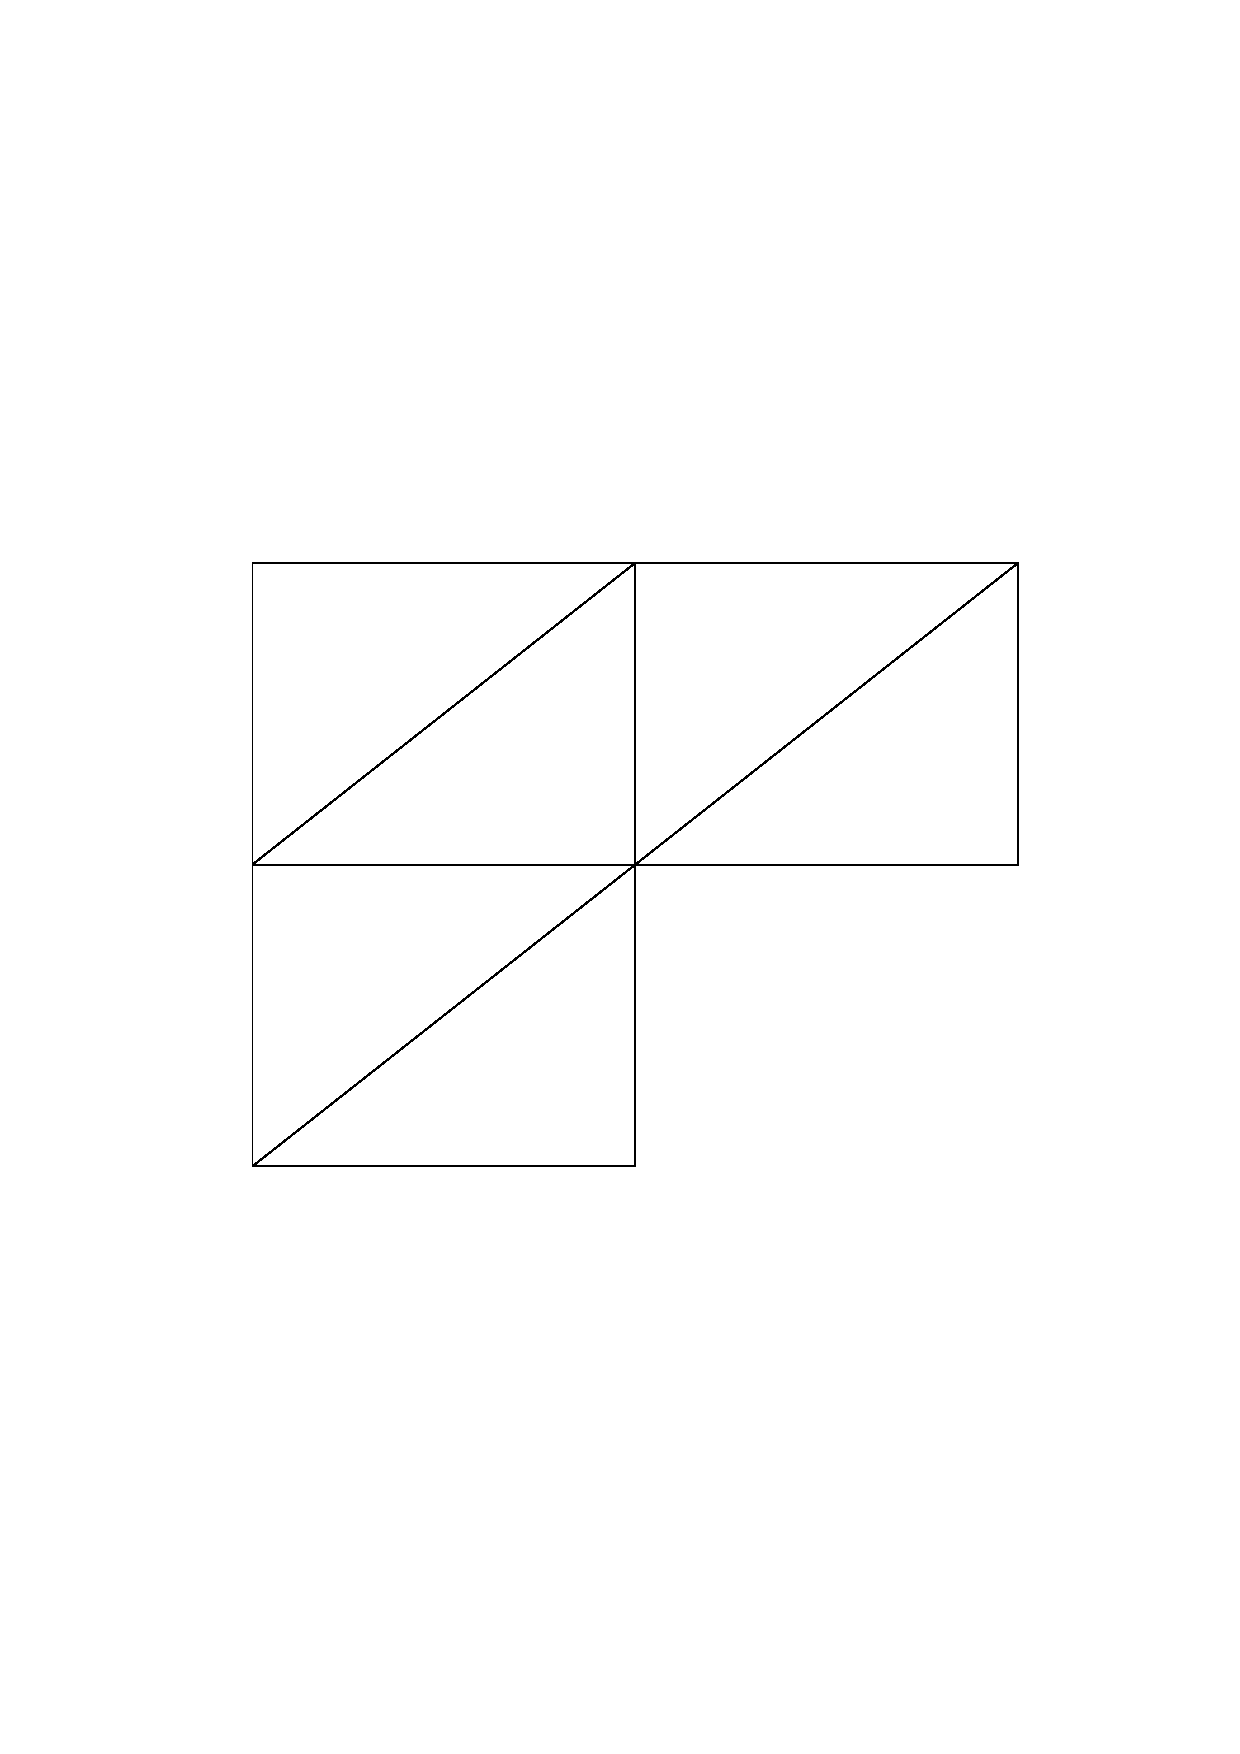
\includegraphics[width=0.9\textwidth]{images/sect_ImplementedProblems_Lshape.pdf}
\end{minipage}
\begin{minipage}{0.85\textwidth}
The L-shaped domain $\Omega=[-1,1]^2\setminus\{(0,1]\times(0,-1]\}$ with pure Dirichlet-boundary.
\end{minipage}
\bigskip

\noindent\emph{LshapeNeumann}\smallskip\\
\begin{minipage}{0.14\textwidth}
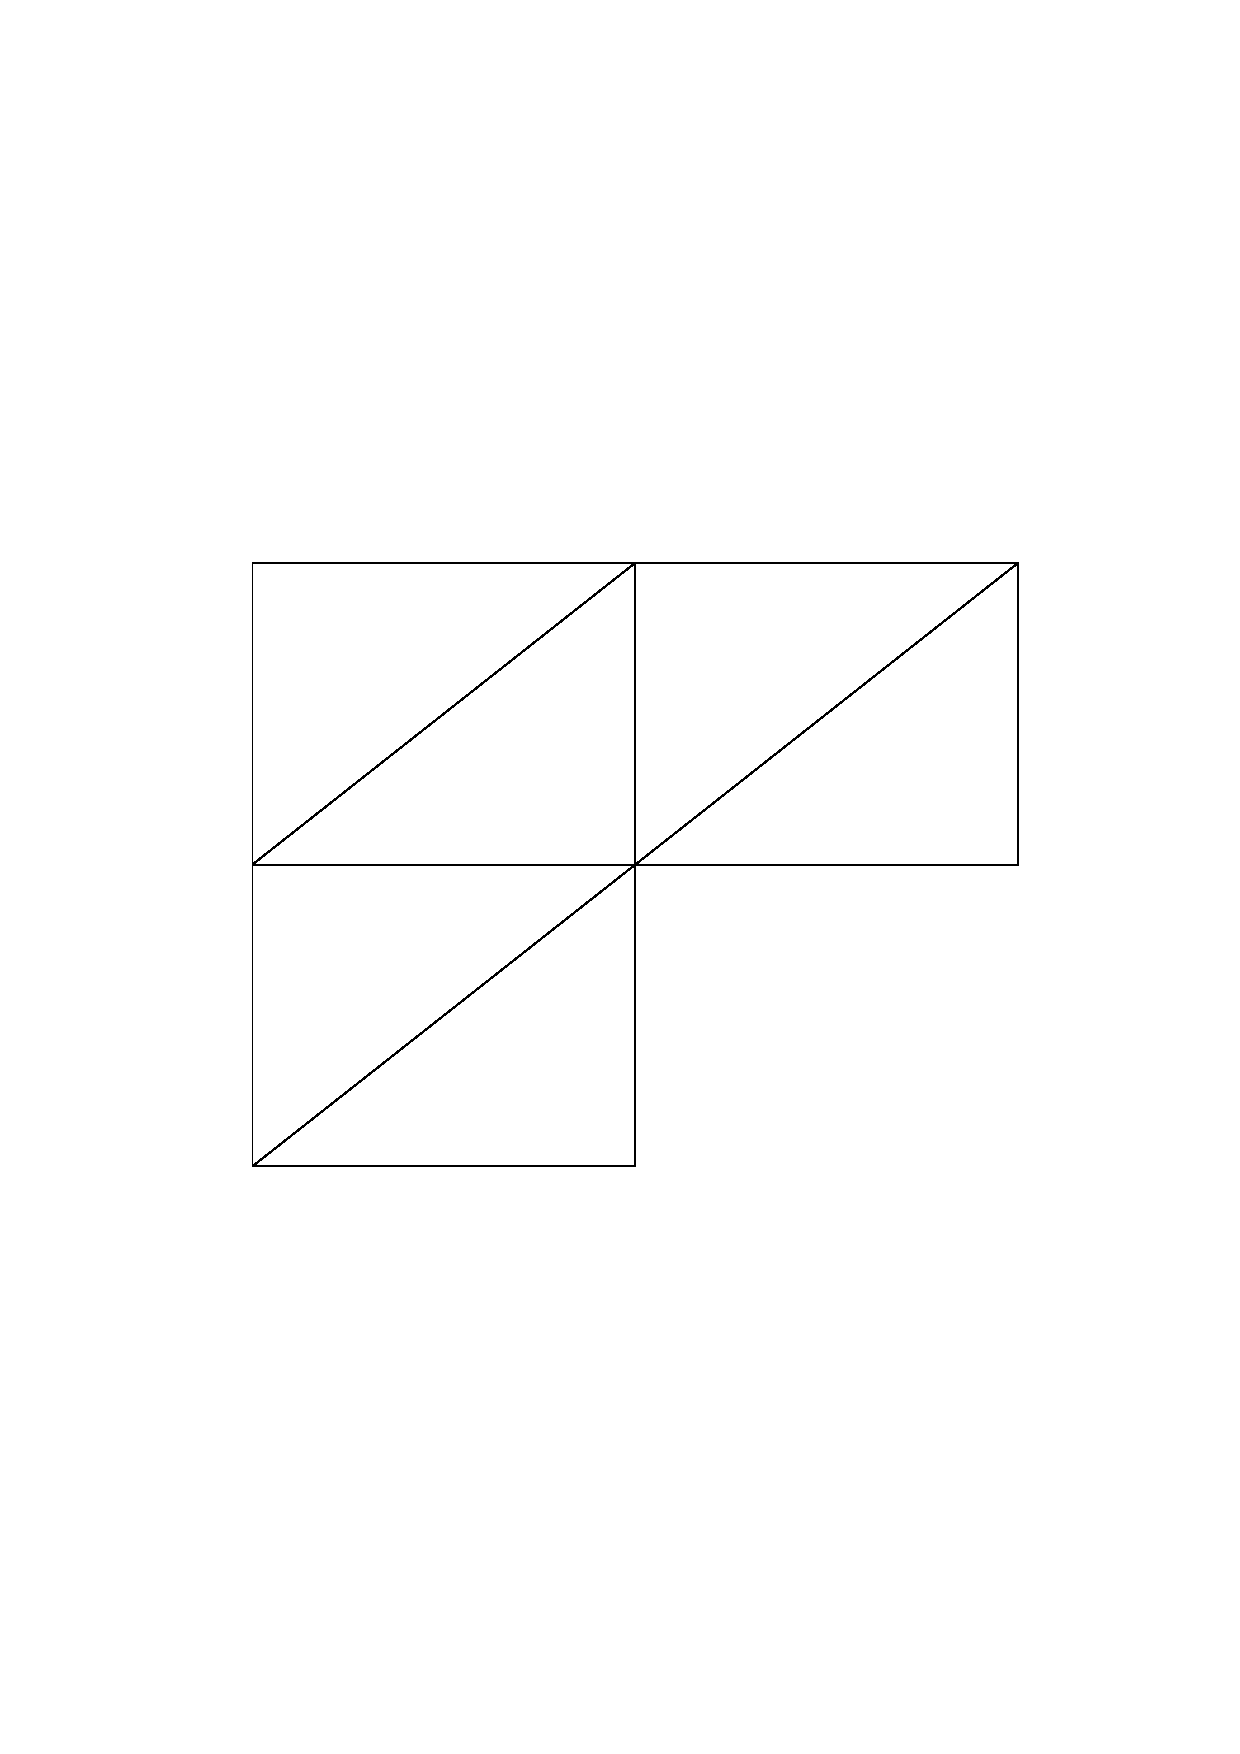
\includegraphics[width=0.9\textwidth]{images/sect_ImplementedProblems_Lshape.pdf}
\end{minipage}
\begin{minipage}{0.85\textwidth}
The domain is the L-shape domain with Neumann boundary.  $\Gamma_D=\left\{\conv\{(0,0),(1,0)\}\cup\conv\{(0,0),(0,-1)\}\right\}$.
\end{minipage}
\bigskip

\noindent\emph{Lshape3}\smallskip\\
\begin{minipage}{0.14\textwidth}
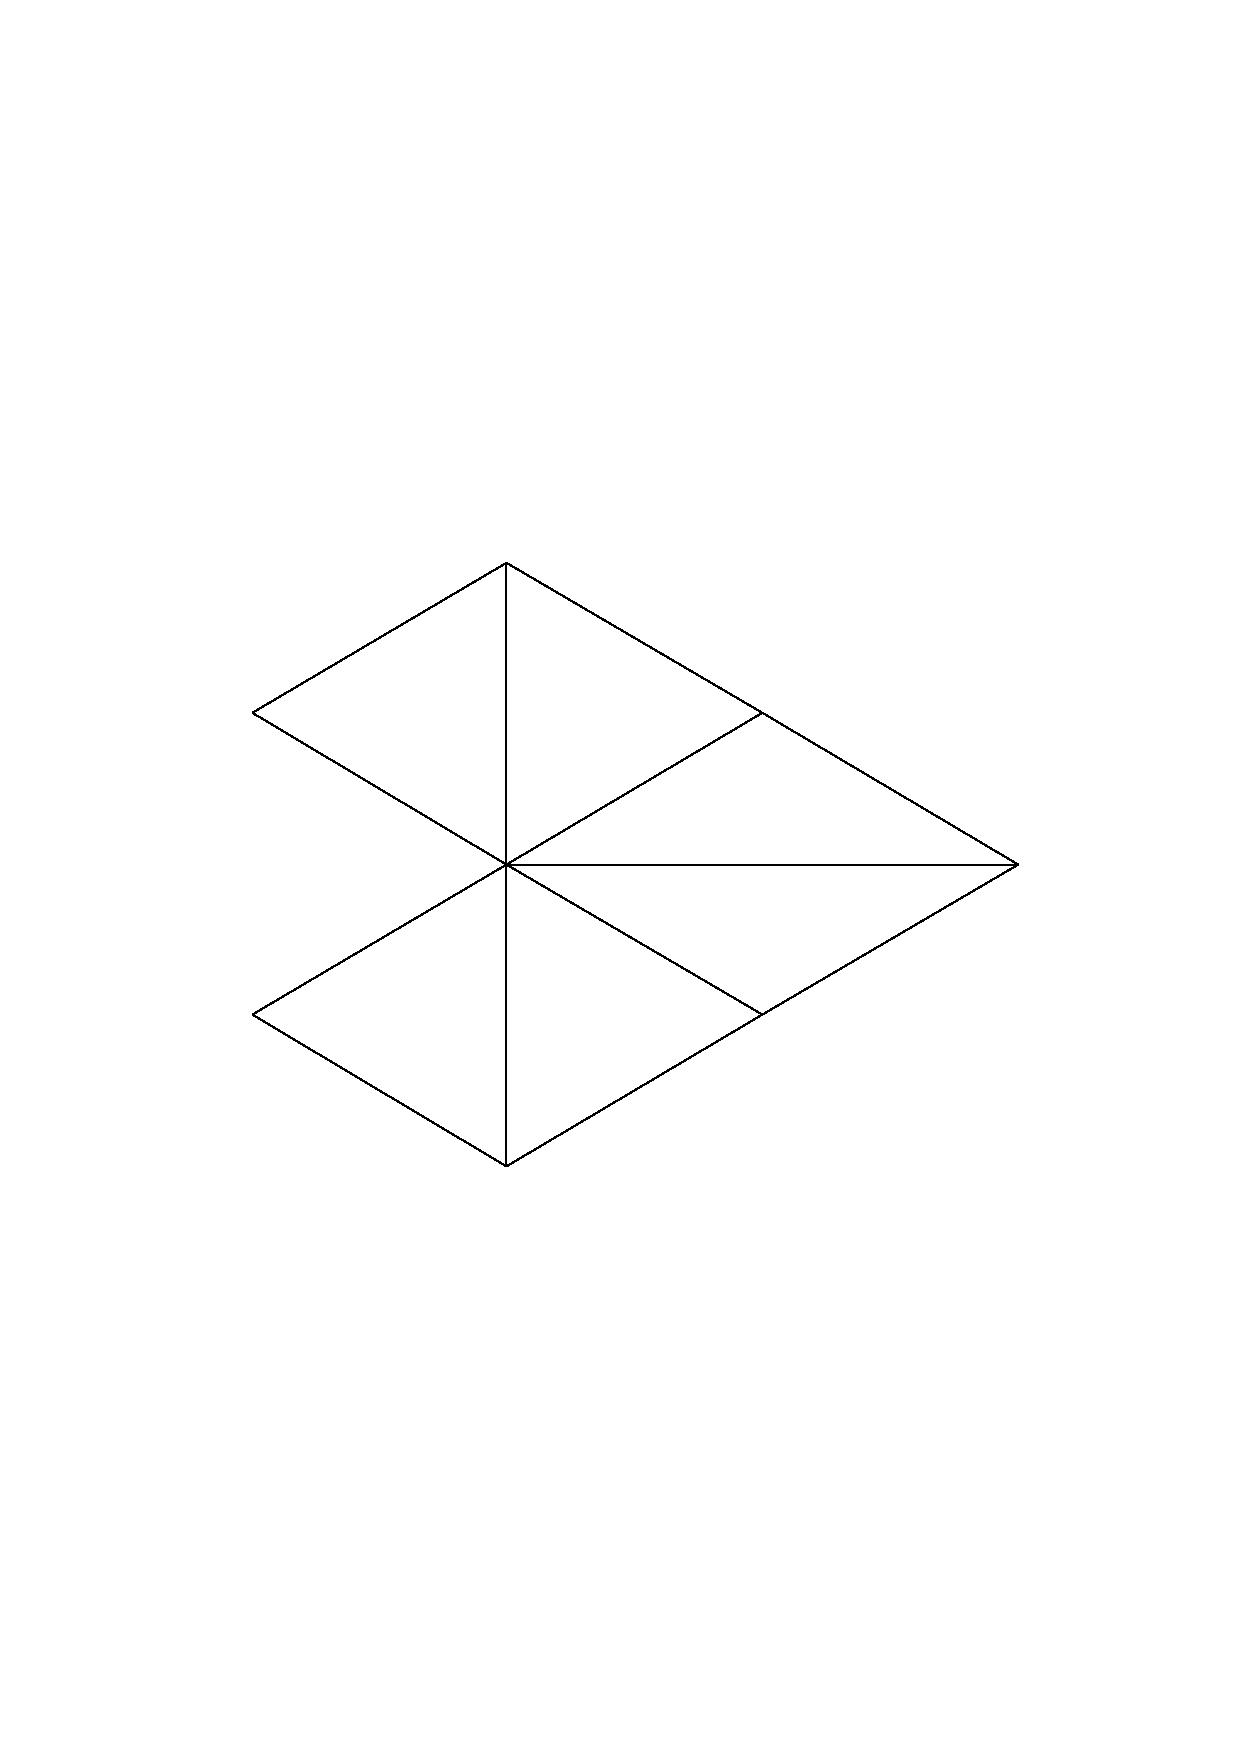
\includegraphics[width=0.9\textwidth]{images/sect_ImplementedProblems_Lshape3.pdf}
\end{minipage}
\begin{minipage}{0.85\textwidth}
Lshape3 is a rotated version of Lshape. Here the boundary of the rotated L-shaped domain is not axis parallel anymore.
\end{minipage}
\bigskip

\noindent\emph{Lshape3Neumann}\smallskip\\
\begin{minipage}{0.14\textwidth}
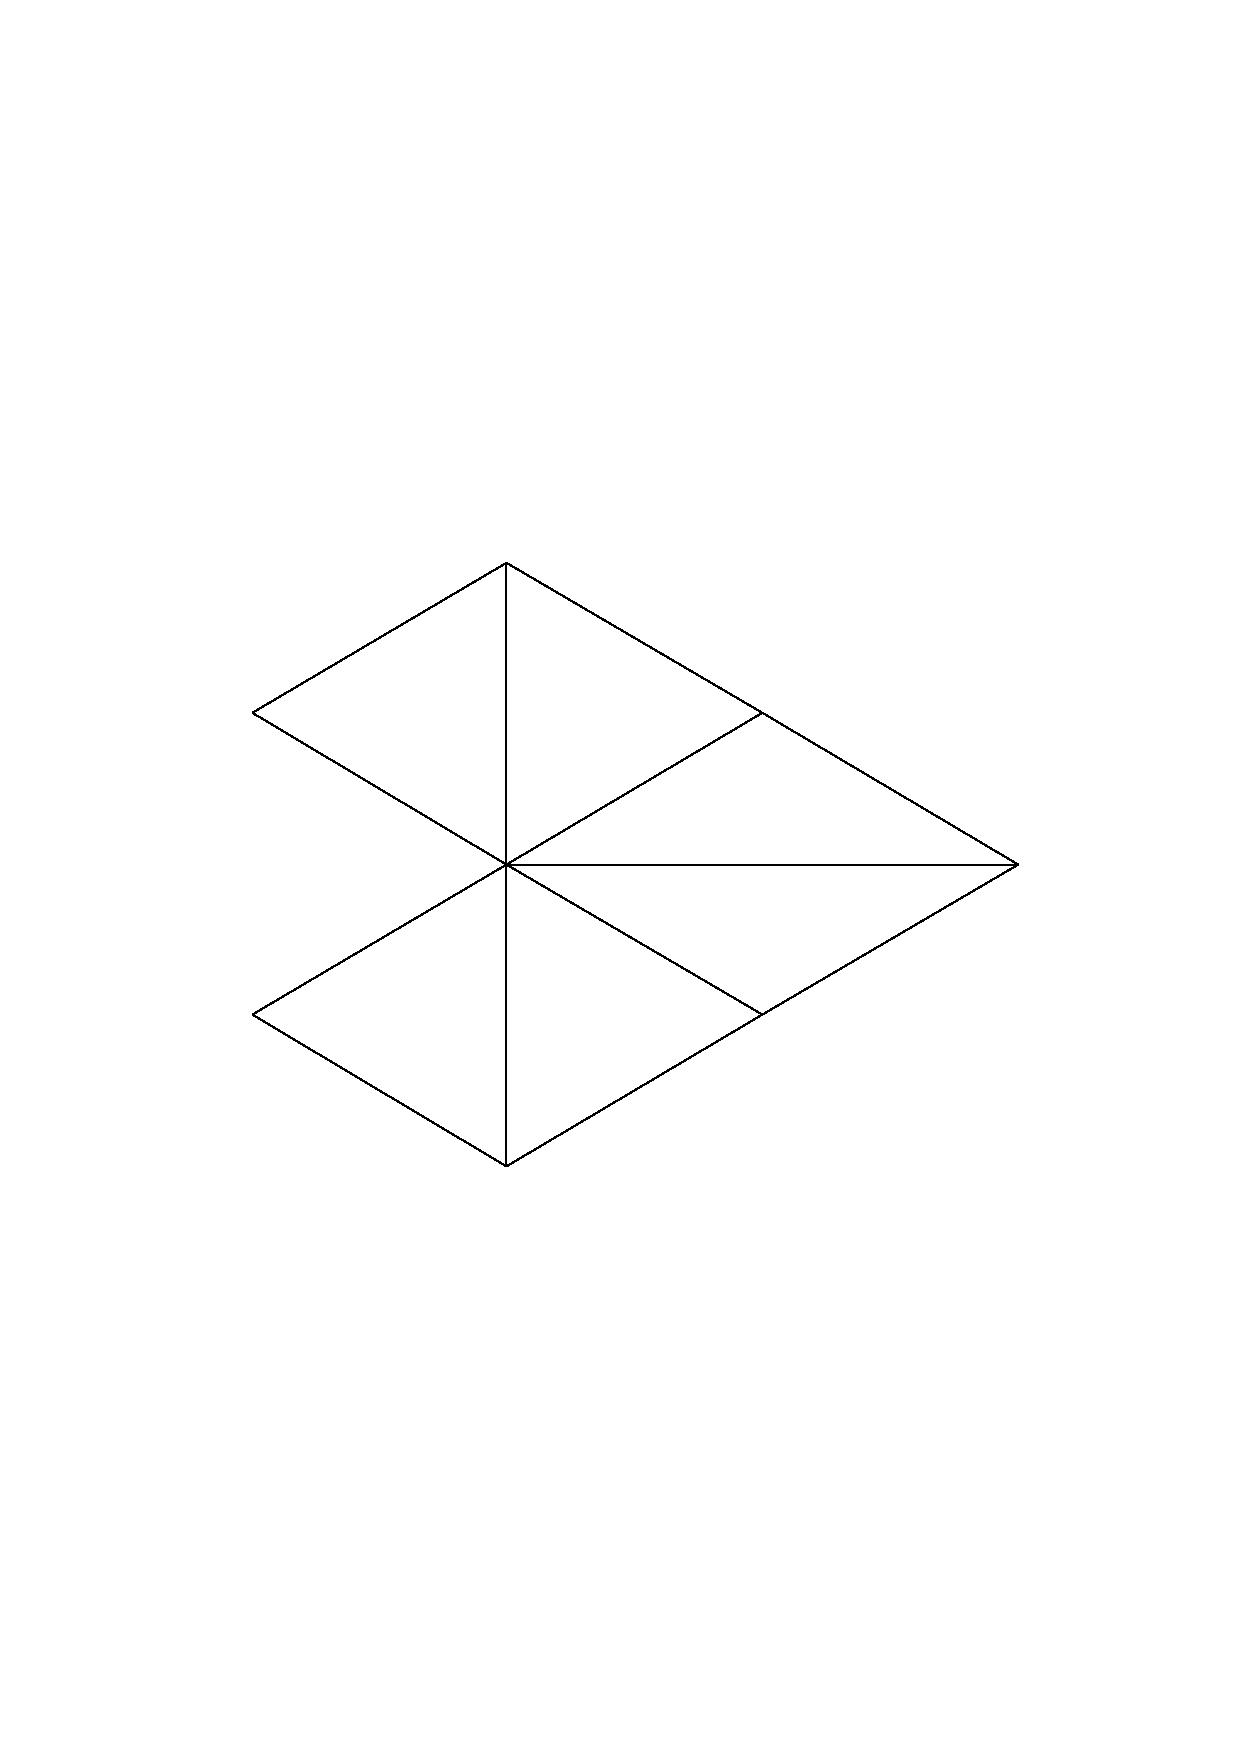
\includegraphics[width=0.9\textwidth]{images/sect_ImplementedProblems_Lshape3.pdf}
\end{minipage}
\begin{minipage}{0.85\textwidth}
Lshape3Neumann is a rotated version of LshapeNeumann.
\end{minipage}
\bigskip

\noindent\emph{Cooks}\smallskip\\
\begin{minipage}{0.14\textwidth}
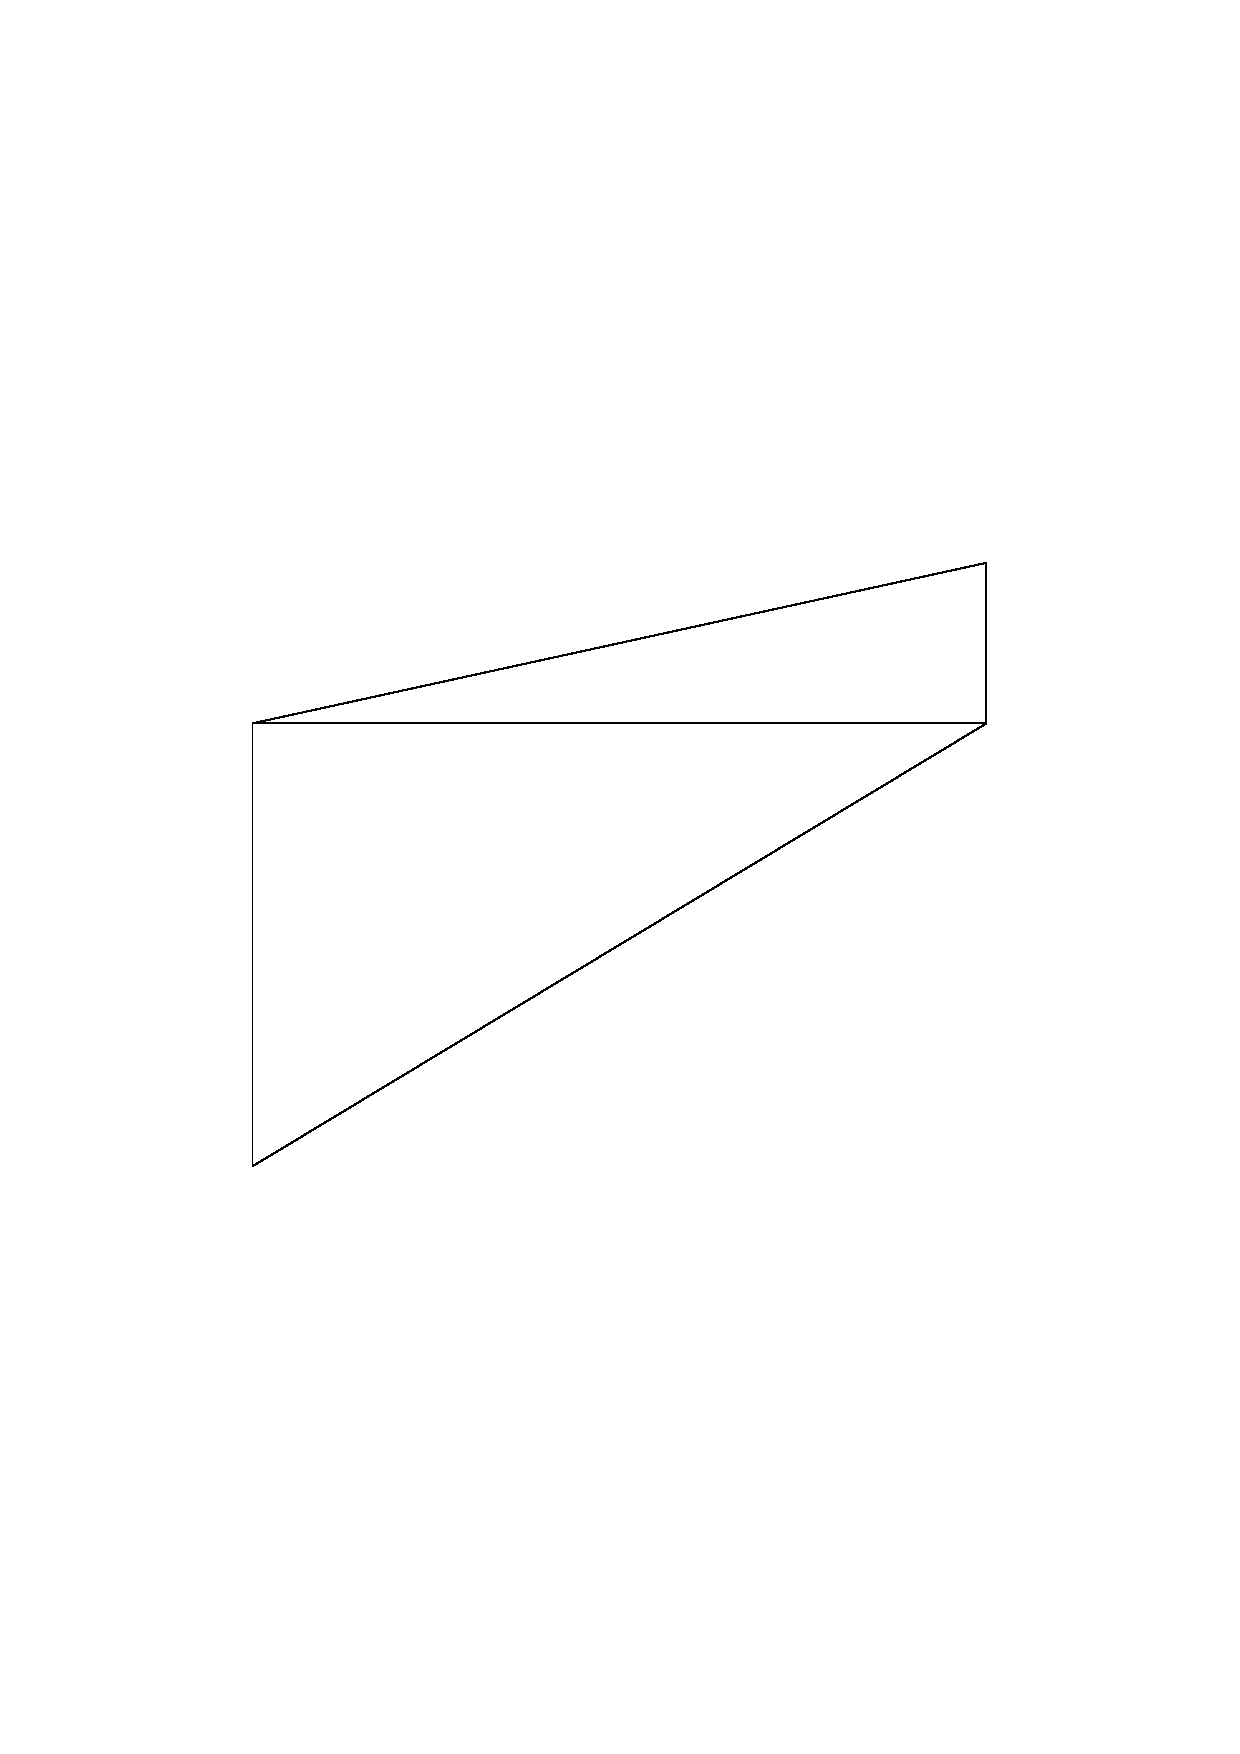
\includegraphics[width=0.9\textwidth]{images/sect_ImplementedProblems_Cooks.pdf}
\end{minipage}
\begin{minipage}{0.85\textwidth}
Geometry for the Cook's membrane problem in elasticity. $\Omega=\conv\{(0,0),(48,44),(48,60),(0,44)\}$. The Dirichlet boundary $\Gamma_D$ is $\conv\{(0,0),(0,44)\}$. Thus the Neumann boundary is $\partial\Omega\setminus\Gamma_D$.
\end{minipage}
\bigskip

\noindent\emph{HexagonalSlit}\smallskip\\
\begin{minipage}{0.14\textwidth}
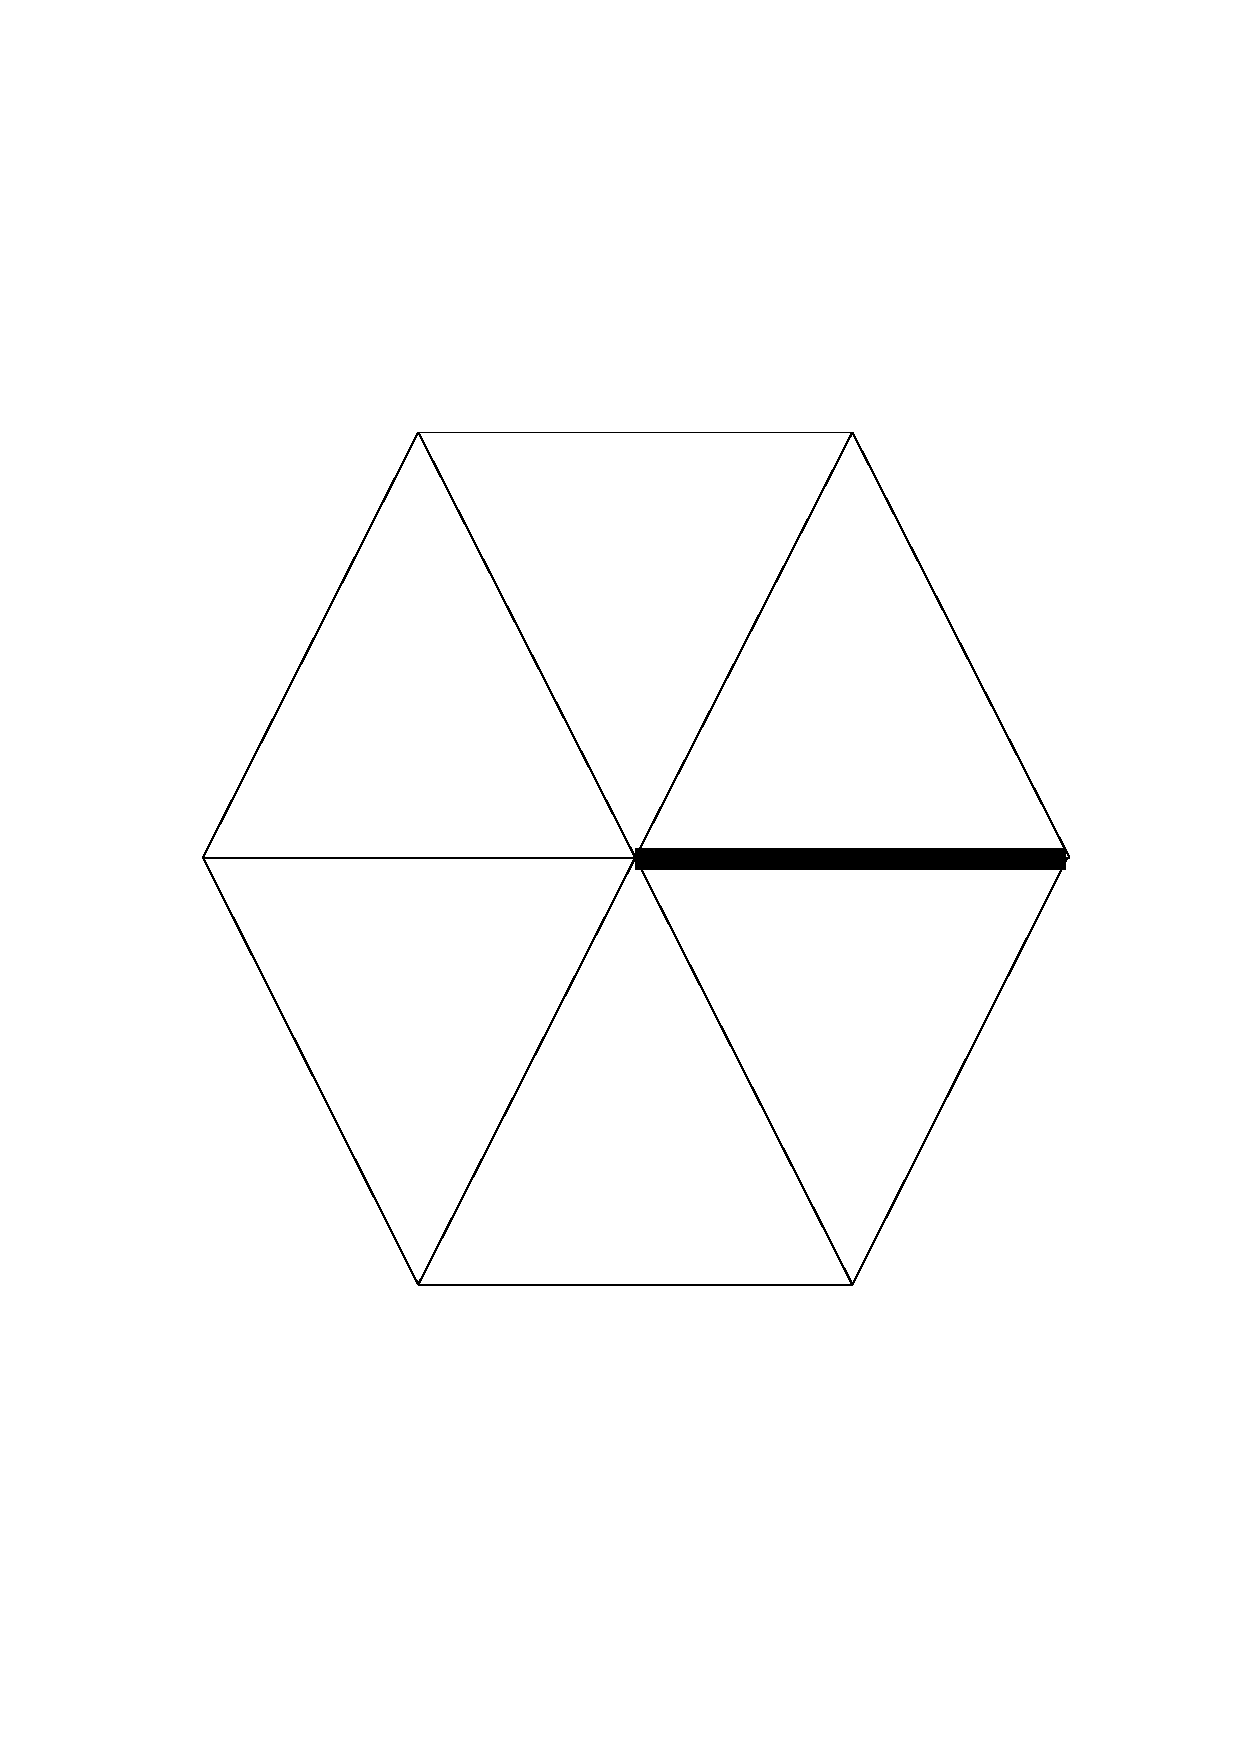
\includegraphics[width=0.8\textwidth]{images/sect_ImplementedProblems_HexagonalSlit.pdf}
\end{minipage}
\begin{minipage}{0.85\textwidth}
We have defined a hexagon $\Omega\subset[-1,1]^2$ which is slitted in $\{0\}\times[0,1]$. The slit is approximated by adding an additional node through a small, numerically insignificant, perturbation of the node $(0,1)$. The slitted hexagon is an example for a non-Lipschitz domain with pure Dirichlet boundary.
\end{minipage}
\bigskip
%\subsection{Eigenwert Probleme}
Gesucht sind die Eigenwerte $\omega$ und Eigenfunktionen $u$, $\lVert u\rVert_{L^2}=1 $, des elliptischen Eigenwertproblems
\begin{align*}
  -div(\kappa(x)\cdot\nabla u) + \lambda(x)\cdot\nabla u + \mu(x)\cdot u &= \omega u \\
\nonumber
  u &= u_D \hbox{, auf } \Gamma_D \\
  \frac{\partial u}{\partial \eta} &= g \hbox{, auf } \Gamma_N\; .
\end{align*}
Damit das \FFW alle Einstellungen in Bezug auf Eigenwertprobleme
�bernimmt muss zuerst
\begin{verbatim}
p.params.problem.type = 'eigenvalue';
p.params.solver = 'eigenvalue';
\end{verbatim}
gesetzt werden. Dies kann auch mittels eines Aufrufs von
\begin{verbatim}
p = configureP(pdeSolver,problem,mark,maxNrDoF,[],'eigenvalue');
\end{verbatim}
geschehen.\\
In der Datei \path{startEigenvalue.m} wurden alle Einstellungen schon vorgenommen. Dort stehen auch ein paar Problemstellungen zur Auswahl.

\subsubsection{Lineares Gleichungssystem l�sen}
\hspace{0cm}

\medskip
\noindent
\textbf{Datei:} \path{algorithms/linSysSolvers/eigenvalue/solve.m}\\[1.5ex]
Durch Finite Element Discretisierung des Eigenwert Problems erh�lt man ein verallgemeinertes Eigenwertproblem f�r Matrizen.
\begin{equation*}
A u = \omega B u\;
\end{equation*}
Es wird die Funktion \code{eigs} von MATLAB benutzt die unter Anderem auf das Packet ARPACK zur�ckgreift. Der Parameter \code{p.params.curEigenvalue} gibt dabei an, welcher Eigenwert berechnet werden soll. \code{eigs} berechnet alle \code{curEigenvalue} kleinsten Eigenwerte und Eigenfunktionen. Da das Gitter aber nur f�r den einen Eigenwert bzw. Eigenfunktion adaptiv verfeinert werden kann, wird auch nur dieser gespeichert. Die Anzeige wird vorher auf 'stumm' gestellt.
\begin{verbatim}
options.disp = 0;
[V,D] = eigs(A(freeNodes,freeNodes),B(freeNodes,freeNodes),...
             curEigenvalue,'sm',options);
\end{verbatim}

\subsubsection{PDESolver}
Zur Zeit ist nur die P1-FEM implementiert. Diese befindet sich im Ordner \path{/PDESolvers/P1-Eigenvalue}.
\begin{verbatim}
p.params.pdeSolver = 'P1-Eigenvalue';
\end{verbatim}
Die Steifigkeitsmatrix A und die Massenmatrix B wird dabei in
\begin{verbatim}
p.level(end).A
p.level(end).B
\end{verbatim}
gespeichert.

\subsubsection{Problem}
Zwei Problemdefinitionen stehen aktuell zur Verf�gung. Zum einen das Laplace Problem auf dem Quadrat f�r homogene Randdaten und zum anderen das Laplace Problem auf dem L-Shape ebenfalls mit homogenen Randdaten. Diese befinden sich im Verzeichniss \path{/problems/eigenvalue/}
\begin{verbatim}
p.params.problem.name = 'Laplace-Square-exact';
p.params.problem.name = 'Laplace-Lshape';
\end{verbatim}

\subsubsection{Parameter}
\hspace{0cm}

\medskip \noindent
\textbf{p.params.curEigenvalue}\\
Gibt an welcher Eigenwert ausgehend vom kleinsten Eigenwert berechnet werden soll (Default = 1).

\medskip \noindent
\textbf{p.params.modules.mark.refineFirstLevel}\\
Um gr�ssere Eigenwerte berechnen zu k�nnen muss auch die Matrix gross genug sein. D.h. es m�ssen gen�gend innere Knoten vorhanden sein. Um das zu garantieren kann mit diesem Parameter angegeben werden wie oft das Gitter uniform verfeinert wird, bevor die erste L�sung berechnet wird (Default = 1).

\subsubsection{ErrorType}
Zus�tzlich zu den anderen Typen ('estimatedError', 'L2error', 'H1semiError') steht bei Eigenwert Problemen noch der Typ 'eigenvalueError' zur Verf�gung. So l�sst sich mittels
\begin{verbatim}
p = show('drawError_eigenvalueError',p);
\end{verbatim}
der exakte Fehler des Eigenwertes in einer Graphik mit logarithmischen Skalen darstellen. Dazu mus vorher der exakte Eigenwert definiert worden sein.
\begin{verbatim}
p.problem.eigenvalue_exact = exakter Eigenwert;
\end{verbatim}


\section{Data Structures}
\label{sect:DataStructures}
%In algorithms/enum sind die Funktionen, die alle im
%\FFW ben\"otigten Gitterinformationen und die
%lokalen Gradienten f\"ur $P_1$ und $CR$
%Basisfunktionen auf jedem Element berechnen.
%
%Die Informationen werden in Matrizen eingetragen, so dass die Zeile
%und/oder Spalten den Nummern der Knoten, Elemnte, Kanten usw.
%entsprechen, f\"ur die man die entsprechende Information erhalten
%m\"ochte. Ist f\"ur die Knoten, Elemente, Kanten usw. keine
%Information vorhanden wird eine Null eingetragen. Zum Beispiel, wenn
%eine Kante eine Randkante ist und es somit nicht zwei Elemente gibt,
%die sie teilen. Die Namen sind so zu verstehen, dass die n f\"ur \textbf{N}odes, e f\"ur 
%\textbf{e}lements und ed f\"ur \textbf{ed}ges steht. So dass also e4ed also hei\"st 
%\"'elements for edges\"'. Bei Daten, die den Dirichlet bzw. den Neumannrand betreffen, 
%wird kurz Db bzw. Nb geschrieben. Im folgenden werden diese Namen, sowie die Abk\"urzungen 
%nrNodes f\"ur die Anzahl der Knoten, nrElems f\"ur die Anzahl der Elemente usw. benutzt.
%
%Die gesamten Gitterinforamtionen Informationen werden aus den angegebenen Triangulierungsdaten n4e,
%c4n, Db, Nb generiert. Dabei werden allerdings nicht alle Informationen aus diesen Angaben direkt
%erzeugt. So wird z.B. e4n aus n4e, ed4n aus e4n und Ed4e dann aus ed4e und n4e erzeugt.

In \path{./algorithms/enum} are the functions which calculate all grid information 
needed in the \FFW, e.g. area of elements, length of edges, outer unit normals 
of the boundary, and the local gradients for $P_1$ and $P_1^{NC}$ basis functions.

This information is stored in matrices. In these matrices a row or column number 
corresponds to the number of an element, node, edge etc. If there is no information 
on an element, node, edge etc. the corresponding entry is zero. For example a boundary 
edge will have only one none zero entry in e4ed, since there is only one element 
which contains it.


In the names of the data matrices \textbf{e} stands for \textbf{e}lements, \textbf{n} for \textbf{n}odes
\textbf{ed} for \textbf{ed}ges, \textbf{Db} for \textbf{D}irichlet\textbf{b}oundary, \textbf{Nb} 
\textbf{N}eumann\textbf{b}oundary and \textbf{4} means '\textbf{for}'. E.g., the matrix e4ed contains elements
for an edge. In the following these names are used as well as the abriviations nrElems, 
nrNodes etc., standing for number of elements, number of Nodes etc.

In a triangulation in the \FFW the geometric primitives (elements, nodes and edges) are 
numbered uniquely. Dirichlet and Neummann edges are also numbered in this way. The numbering of 
elements, nodes, Dirichlet and Neumann edges is defined by n4e, c4n, Db and Nb, respectively, 
whereas the edge numbers are created in path{./enum/getEd4n}. All the other information (e.g. Normals, Tangents) 
is not numbered and is used as attributes of the information above.

For the geometric primitive one has not only a global number, but most times also a local one. 
For example the global number of a node is defined by the row number in c4n, and for each 
element its nodes are locally numbered from one to three by there order in the 
corresponding row in n4e.

To calculate all the grid information the only initial data needed is n4e, c4n, Db, Nb.
Please note that not all information is calculated using directly the initial data. For
example e4n needs only the information in n4e but ed4n is created using the information 
in e4n.

%Die anzugebenden Triangulierungsdaten sind:
%
%\begin{longtable}{p{0.1\textwidth}p{0.35\textwidth}p{0.45\textwidth}}
%c4n & $nrNodes \times 2$ & Jede Zeile definiert einen Knoten mit den
%eingetragenen Werten als Koordinaten. Die erste Spalte enth�t dabei
%die x-Koordinaten und die zweite die y-Koordinaten. Die Knotennummer
%ist die Nummer der Zeile.\\
%n4e&$nrElems \times 3$&Jede Zeile definiert ein Element mit den
%eingetragenen Knoten als Eckpunkte. Die drei Eckpunkte sind gegen
%den Uhrzeigersinn anzugeben. Die Elementnummer ist die Nummer der
%Zeile.\\
%Db&$nrDirichletEdges \times 2$&Jede Zeile definiert die Kante zwischen den
%eingetragenen Knotennummern als Dirichletkante. Die Knotennummern in
%einer Zeile sind in der gleichen Reihenfolge wie in dem zugeh\"origen Dreieck in n4e anzugeben.\\
%Nb&$nrNeumannEdges \times 2$&Jede Zeile definiert die Kante zwischen den
%eingetragenen Knotennummern als Neumannkante. Die Knotennummern in
%einer Zeile sind in der gleichen Reihenfolge wie in dem zugeh\"origen Dreieck in n4e anzugeben.
%\end{longtable}


The initial data consists of:

\begin{longtable}{p{0.1\textwidth}p{0.35\textwidth}p{0.45\textwidth}}
Name&Dimension&Description\\ \hline
c4n & $nrNodes \times 2$ & Each row defines a node at the coordinates given by the values. 
Where the first column contains the x-coordinate and the second the y-coordinate. The number 
of the defined node is the number of the row.\\
n4e&$nrElems \times 3$&Each row defines an element with the nodes corresponding to the entries 
as vertices. The vertices have to be entered counter clockwise. The number 
of the defined element is the number of the row.\\
Db&$nrDirichletEdges \times 2$&Each row defines the edge between the two nodes corresponding 
to the entries as a Dirichlet edge. In each row the nodes have to be in the same order as in 
the corresponding element.\\
Nb&$nrNeumannEdges \times 2$&Each row defines the edge between the two nodes corresponding 
to the entries as a Neumann edge. In each row the nodes have to be in the same order as in 
the corresponding element.
\end{longtable}

%Die folgende Grafik zeigt mit welchen Matrizen man von einer Information zu einer anderen bergehen kann.
%Um z.B. alle Kanten fr ein Element zu erhalten, muss man die entsprechende Zeile in ed4e aufrufen.
%



The following figure shows how one can get from one geometric primitive to another one. To get for example 
all edges for one element just look at the corresponding row in ed4e.

\begin{figure}[ht!]
\begin{center}
\setlength{\unitlength}{3.5cm}
\begin{picture}(1.5,1)
\put(0,0){\line(1,0){1.2}}
\put(0,0){\line(2,3){0.6}}
\put(1.2,0){\line(-2,3){0.6}}
\put(-0.3,-0.1){\textbf{N}odes}
\put(1.25,-0.1){\textbf{Ed}ges}
\put(0.4,0.95){\textbf{E}lements}
\put(0.105,0.2){\vector(2,3){0.4}}
\put(0.1,0.5){e4n}
\put(0.5,0.7){\vector(-2,-3){0.4}}
\put(0.32,0.35){n4e}
\put(0.735,0.74){\vector(2,-3){0.4}}
\put(1,0.4){ed4e}
\put(1.05,0.18){\vector(-2,3){0.4}}
\put(0.6,0.46){e4ed}
\put(0.16,0.03){\vector(1,0){0.9}}
\put(0.6,0.05){ed4n}
\put(1,-0.03){\vector(-1,0){0.9}}
\put(0.4,-0.11){n4ed}

\end{picture}
\end{center}
\caption{A diagram illustrating mesh dimension traversal.}\label{sect:DataStructures.fig.DataRelations}
\end{figure}



%An Gitterinformationen werden erzeugt (jeweils von der Funktion
%GetINFORMATION):
%
%\begin{longtable}{p{0.2\textwidth}p{0.25\textwidth}p{0.45\textwidth}}
%Name&Dimension&Beschreibung\\ \hline
%e4n&$nrNodes \times nrNodes$&Jeder Eintrag (j,k) enth\"alt die Elementnummer 
%des Elementes, das die Knoten j und k gegen den Uhrzeigersinn als Eckpunkte hat\\
%ed4n&$nrNodes \times nrNodes$&Jeder Eintrag (j.k) enth\"alt die Kantennummer 
%der Kante, die die Knoten j und k beinhaltet\\
%ed4e&$nrElems \times 3$&Jede Zeile enth\"alt die Kantennummern des entsprechenden 
%Elemnts gegen den Uhrzeigersinn entsprechend der Reihenfolge der Knoten in n4e\\
%n4ed&$nrEdges \times 2$&Jede Zeile enth\"alt die Knotennummern der Knoten, die 
%die entsprechende Kante beinhaltet\\
%e4ed&$nrEdges \times 2$&Jede Zeile enth\"alt die Elementnummern der Elemente, 
%die die entsprechende Kante teilen bzw. enthalten in absteigender Reihenfolge\\
%DbEdges&$nrDbEdges \times 1$&Jede Zeile enth\"alt die Kantennummer einer Dirchletkante in der Reihenfolge von Db\\
%NbEdges&$nrNbEdges \times 1$&Jede Zeile enth\"alt die Kantennummer einer Neumannkante in der Reihenfolge von Nb\\
%area4e&$nrElems \times 1$&Jede Zeile enth\"alt die Fl\"ache f\"ur das entsprechende Element\\
%midpoint4e&$nrElems \times 2$&Jede Zeile enth\"alt die Koordinaten des Mittelpunktes des entsprechenden Elements\\
%midpoint4ed&$nrEdges \times 2$&Jede Zeile enth\"alt die Koordinaten des Mittelpunktes der entsprechende Kante\\
%tangents4e&$3 \times 2 x nrElems$&Jede $3\times2$ Matrix enth\"alt die Koordinaten der drei Einheitstangenten des entsprechenden Elements\\
%normals4e&$3 \times 2 nrElems$&Jede $3\times2$ Matrix enth\"alt die Koordinaten der drei \"au�ren Einhietsnormalen des entsprechenden Elements\\
%normals4DbEd&$nrDbEdges \times 2$&Jede Zeile enth\"alt die Koordinaten der \"au�ren Einheitsnormalen an der entsprechenden Dirichletkante\\
%normals4NbEd&$nrNbEdges \times 2$&Jede Zeile enth\"alt die Koordinaten der \"au�ren Einheitsnormalen an der entsprechenden Neumannkante\\
%length4ed&$nrEdges \times 1$&Jede Zeile enth\"alt die L\"ange der entsprechenden Kante\\\
%area4n&$nrNodes \times 1$&Jede Zeile enth\"alt die Fl\"ache des Knotenpatches des entsprechenden Knotens\\
%angles4e&$nrElems \times 3$&Jede Zeile enth\"alt die drei Innenwinkel (in radiant) des Elementes in der Reihenfolge der zugeh\"origen Knoten in n4e\\
%angle4n&$nrNodes \times 1$&Jede Zeile enth\"alt die Summe der an den entsprechenden Knoten anliegenden Innenwinkel\\
%grad4e&$3 \times 2 \times nrElems$& Jede Zeile der $3\times2$-Matrizen enth\"alt den lokalen Gradienten einer $P_1$-Basisfunktion.\\
%gradNC4e&$3 \times 2 \times nrElems$& Jede Zeile der $3\times2$-Matrizen enth\"alt den lokalen Gradienten einer $CR$-\-Basisfunktion.\\
%\end{longtable}

The created grid information is (they are always created by the function get\textit{Name}):

\begin{longtable}{p{0.2\textwidth}p{0.25\textwidth}p{0.45\textwidth}}
Name&Dimension&Description\\ \hline
e4n&$nrNodes \times nrNodes$&Each entry (j,k) contains the number of the element which has the nodes j and k 
counter clockwise as vertices.\\
ed4n&$nrNodes \times nrNodes$&Each entry (j,k) contains the number of the edge between the nodes j and k.\\
ed4e&$nrElems \times 3$&Each row contains the edge numbers of the corresponding element.\\
n4ed&$nrEdges \times 2$&Each row contains the node numbers of the corresponding edge.\\
e4ed&$nrEdges \times 2$&Each row contains the element numbers of the elements sharing the corresponding edge 
in descending order.\\
DbEdges&$nrDbEdges \times 1$&Each row contains the number of a Dirichlet edge corresponding to the row in Db.\\
NbEdges&$nrNbEdges \times 1$&Each row contains the number of a Neumann edge corresponding to the row in Nb.\\
area4e&$nrElems \times 1$&Each row contains the area of the corresponding element.\\
midpoint4e&$nrElems \times 2$&Each row contains the coordinates of the midpoint of the corresponding element.\\
midpoint4ed&$nrEdges \times 2$&Each row contains the coordinates of the midpoint of the corresponding edge.\\
tangents4e&$3 \times 2 \times nrElems$&Each $3\times2$ matrix contains the coordinates of the three unit tangents of 
the corresponding element.\\
normals4e&$3 \times 2 \times nrElems$&Each $3\times2$ matrix contains the coordinates of the three outer unit normals of 
the corresponding element.\\
normals4DbEd&$nrDbEdges \times 2$&Each row contains the coordinates of the outer unit normals of 
the corresponding Dirichlet edge.\\
normals4NbEd&$nrNbEdges \times 2$&Each row contains the coordinates of the outer unit normals of 
the corresponding Neumann edge.\\
length4ed&$nrEdges \times 1$&Each row contains the length of the corresponding edge.\\\
area4n&$nrNodes \times 1$&Each row contains the area of the node patch of the corresponding node.\\
angles4e&$nrElems \times 3$&Each row contains the inner angles at each node of the corresponding element 
in the order given in the rows of n4e.\\
angle4n&$nrNodes \times 1$&Each row contains the sum of all inner angles at the corresponding node.\\
grad4e&$3 \times 2 \times nrElems$&Each $3\times2$ matrix contains the three local gradients of the three $P1$ 
basis functions not completely zero on the corresponding element.\\
gradNC4e&$3 \times 2 \times nrElems$&Each $3\times2$ matrix contains the three local gradients of the three $CR$ 
basis functions not completely zero on the corresponding element.\\
\end{longtable}

%Anhand der folgenden grafik sollen kurz ein paar Beispiele die Datenstrukturen erl\"autern. Die r\"omischen Ziffern in
%einer Raute sind hier die Nummern des jeweiligen Elements, die arabischen Zahlen in Kreisen die Nummern der Knoten und die kursiven arabischen Zahlen in den K\"astchen die Nummern der Kanten.

The following figure shows a triangulation of two triangles generated by the \FFW. The numbering is used to illustrate the
structure of the data created in \path{./algorithms/enum} by means of some examples. The latin numbers in rhombuses are the element numbers, the numbers in circles are the node numbers and the cursive numbers in rectangles are the edge numbers.

\begin{figure}[h!]
\vspace{3ex}
\begin{center}
\setlength{\unitlength}{4cm}
\begin{picture}(2.2,0.9)
\put(0,0){\line(1,0){1.4}}
\put(0,0){\line(3,4){0.7}}
\put(1.4,0){\line(3,4){0.7}}
\put(0.7,0.93){\line(1,0){ 1.4}}
\put(0.7,0.93){\line(3,-4){0.7}}
\put(0.65,0.3){I}
\put(0.58,0.325){\line(2,3){.08}}
\put(0.58,0.325){\line(2,-3){.08}}
\put(0.74,0.325){\line(-2,-3){.08}}
\put(0.74,0.325){\line(-2,3){.08}}
\put(1.35,0.57){II}
\put(1.30,0.595){\line(2,3){.08}}
\put(1.30,0.595){\line(2,-3){.08}}
\put(1.46,0.595){\line(-2,-3){.08}}
\put(1.46,0.595){\line(-2,3){.08}}
\put(-0.05,-0.1){1}
\put(-0.026,-0.075){\circle{0.1}}
\put(1.4,-0.1){2}
\put(1.424,-0.075){\circle{0.1}}
\put(0.65,0.96){4}
\put(0.676,0.985){\circle{0.1}}
\put(2.1,0.96){3}
\put(2.125,0.985){\circle{0.1}}
\put(0.7,-0.08){\it 1}
\put(0.66,-0.09){\line(1,0){0.13}}
\put(0.66,-0.09){\line(0,1){0.09}}
\put(0.79,-0.09){\line(0,1){0.09}}
\put(1.74,0.39){\it 2} 
\put(1.78,0.32){\line(3,4){0.09}}
\put(1.78,0.32){\line(-4,3){0.09}}
\put(1.87,0.44){\line(-4,3){0.09}}
\put(0.24,0.41){\it 3}
\put(0.17,0.41){\line(3,4){0.09}}
\put(0.17,0.41){\line(4,-3){0.09}}
\put(0.26,0.53){\line(4,-3){0.09}}
\put(1.075,0.47){\it 4}
\put(1.10,0.58){\line(3,-4){0.09}}
\put(1.10,0.58){\line(-4,-3){0.09}}
\put(1.19,0.46){\line(-4,-3){0.09}}
\put(1.4,0.94){\it 5}
\put(1.37,1.02){\line(1,0){0.13}}
\put(1.37,1.02){\line(0,-1){0.09}}
\put(1.50,1.02){\line(0,-1){0.09}}
\end{picture}
\caption{Enumeration of nodes, edges and elements.}
\label{sect:DataStructures.fig.ExampleEnumeration}
\end{center}
\end{figure}

Examples:

This n4e creates a triangulation as shown in the Figure~\ref{sect:DataStructures.fig.ExampleEnumeration}:
\begin{verbatim}
>> n4e
n4e =
     1     2     4
     2     3     4
\end{verbatim}
Note that the order of the nodes is important in e4n but it is not in ed4n. 
\begin{verbatim}
>> e4n(2,4)
ans =
     1
>> e4n(4,2)
ans =
     2
>> ed4n(2,4)
ans =
     4
>> ed4n(4,2)
ans =
     4
\end{verbatim}
One can also get the information for more than one item at a time:
\begin{verbatim}
>> n4ed([3 4],2)
ans =
     4
     4
\end{verbatim}
If there is only one element containing the edge, i.e. the edge is a boundary edge, the second entry is zero:
\begin{verbatim}
>> e4ed([1 4],:)
ans =
     1     0
     2     1
\end{verbatim}
The edges are ordered counter clockwise for each element. The first one in each element is the one 
between the first end the second node (\textbf{not} opposite to the first node): 
\begin{verbatim}
>> ed4e(1,:)
ans =
     1     4     3
\end{verbatim}
\bigskip

{\bf \large Overview of the functions:}\bigskip


{\bf \large getE4n.m}\medskip

The function getE4n returns a $nrNodes \times nrNodes$ sparse matrix. NOTE:
The sparsity constant is bounded due to the used mesh generation. The
input is n4e. In this matrix each entry $(j,k)$ is the number of the
element, whose boundary contains the nodes $j$ and $k$ in
counter clockwise order as vertices or zero if the there is no such
element. Since the nodes in n4e are oriented counter clockwise e4n
gives you the number of the row in which the sequence $j\;k$ is found. Note that 
in this context $k\;i\;j$ also contains the sequence $j\;k$. To find the patch of a node $k$, i.e all
elements containing node $k$, just get the non zero entries of the $k$-th row or column.\\ \medskip

{\bf \large getEd4n.m}\medskip

The function getEd4n returns a symmetric $nrNodes \times nrNodes$
sparse matrix. NOTE: The sparse constant is bounded due to the used mesh generation.
 The input is e4n generated by the function getE4n. The
output matrix ed4n contains the numbers of the edges between two
nodes or zero if the two nodes are not on one edge. In the sense
that for node $j$ and node $k$ the entry $(j,k)$, and $(k,j)$ respectively,
is the corresponding edge number. The numbering of the edges is
arbitrarily generated in this function. The input is n4e.\\ \medskip

{\bf \large getN4ed.m}\medskip

The function getN4ed returns a $nrEdges \times 2$ matrix. the input is
ed4n generated by the function getEd4n. The output matrix contains
in each row the number of the two nodes that are the endpoints of
the edge corresponding to the row number.\\ \medskip

{\bf \large getEd4e.m}\medskip

The function getEd4e returns a $nrElems \times 3$ matrix. The input is n4e
and ed4n produced by the function getEd4n. This matrix contains in
each row $j$ the number of the three edges of element $j$. The edge
numbers are the ones generated  in the function GetEd4n. The edges
are ordered counter clockwise beginning with the edge between the
first and the second node in n4e.\\ \medskip

{\bf \large getE4ed.m}\medskip

The function getE4ed returns a $nrEdges \times 2$ matrix. The input  is e4n
and n4ed produced by the functions getE4n and getN4ed, respectively.
The matrix contains in each row $j$ the element numbers of the elements
which share the edge. If the edge is a boundary edge the second
entry is zero.\\
\medskip

{\bf \large getArea4e.m}\medskip

The function getArea4e returns a $nrElems \times 1$ matrix. The input is
n4e and c4n. The matrix contains in each row $j$ the area of the
element corresponding to the element number $j$. \medskip

{\bf \large getArea4n.m}\medskip

The function getArea4n returns a $nrNodes \times 1$ matrix. The input is
e4n and area4e produced by the functions getE4n and getArea4e,
respectively. The matrix contains in each row $j$ the area of the
patch of node $j$.\\ \medskip

{\bf \large getLength4ed.m}\medskip

The function getLength4ed returns a $nrEdges \times 1$ matrix. The input is
c4n and n4ed produced by the function getN4ed. The matrix contains in each row $j$
the length of the $j$-th edge, according to the edge numbers created in getEd4n.\medskip

{\bf \large getDbEdges.m}\medskip

The function getDbEdges returns a $nrDbEdges \times 1$ matrix. The input is 
Db and ed4n produced by the function getEd4n. The Matrix contains the edge numbers
of the edges belonging to the Dirichlet boundary.\medskip

{\bf \large getNbEdges.m}\medskip

The function getNbEdges returns a $nrNbEdges \times 1$ matrix. The input is 
Nb and ed4n produced by the function getEd4n. The Matrix contains the edge numbers
of the edges belonging to the Neumann boundary.\medskip

{\bf \large getNormals4DbEd.m}\medskip

The function getNormals4DbEd returns a $nrDbEdges \times 2$ matrix. The input 
is c4n and Db. The matrix contains in each row $j$ the two coordinates of the 
outer unit normal at the $j$-th Dirichlet edge, corresponding to the order in DbEdges.\medskip

{\bf \large getNormals4NbEd.m}\medskip

The function getNormals4NbEd returns a $nrNbEdges \times 2$ matrix. The input 
is c4n and Nb. The matrix contains in each row $j$ the two coordinates of the 
outer unit normal at the $j$-th Neumann edge, corresponding to the order in NbEdges.\medskip

{\bf \large getNormals4e.m}\medskip

The function getNormnals4e returns a $3 \times 2 \times nrElems$ matrix. the input is 
c4n, n4e and length4ed and ed4e produced by the functions getLength4ed and getEd4e. The three dimensional
matrix contains in the $j$-th $3 \times 2$ matrix the coordinates of the unit outer normals for 
the three edges of element $j$. The order of the three rows corresponds two the order in ed4e.\medskip

{\bf \large getTangents4e.m}\medskip

The function getNormnals4e returns a $3 \times 2 \times nrElems$ matrix. the input is 
c4n, n4e and length4ed and ed4e produced by the functions getLength4ed and getEd4e. The 
three dimensional matrix contains in the $j$-th $3 \times 2$ matrix the coordinates of the unit tangents in 
counter clockwise direction for the three edges of element $j$, i.e. the direction of the edges. 
The order of the three rows corresponds two the order in ed4e.\medskip

{\bf \large getMidpoint4e.m}\medskip

The function getMidpoint4e returns a $nrElems \times 2$ matrix. The input is c4n and n4e. The matrix 
contains in each row $j$ the coordinates of the midpoint of element $j$.\medskip

{\bf \large getMidpoint4ed.m}\medskip

The function getMidpoint4ed returns a $nrEdges \times 2$ matrix. The input is c4n and n4ed. The matrix 
contains in each row $j$ the coordinates of the midpoint of the $j$-th edge.\medskip

{\bf \large getAngles4e.m}\medskip

The function getAngles4e returns a $3 \times nrElems$ matrix. The input is tangents4e produced by 
the function getTangente4e. The matrix contains in each column $j$ the three interior angles of element 
$j$. The order of the angles correspond to the order of the nodes in n4e, i.e. the angles at the first 
node of each element are in the first row, the one at the second in the second etc.\medskip

{\bf \large getAngle4n.m}\medskip

The function getAngle4n returns a $nrNodes \times 1$ matrix. The input is angles4e, n4e, nrElems and nrNodes 
where angles4e is generated by getAngles4e. The matrix contains in each row $j$ the angle at the node $j$, where 
the angle is 2 $\pi$ for inner nodes and the angle inside the domain and between the two boundary edges 
containing the node for nodes at the boundary.\medskip

{\bf \large getGrad4e.m}\medskip

The function getGrad4e returns a $3 \times 2 \times nrElems$ matrix. the input is c4n n4e and area4e 
produced by the function getArea4e. The three dimensional matrix contains in the $j$-th $3 \times 2$ matrix 
the coordinates of the local gradients of the three $P1$ basis function which are not constantly zero on 
the $j$-th element. The first row in each $3 \times 2$ matrix contains the local gradient of the nodal basis 
function for the first node of the element according to the order in n4e, the second row the one of the 
nodal basis function for the second node etc.\medskip

{\bf \large getGradNC4e.m}\medskip

The function getGrad4e returns a $3 \times 2 \times nrElems$ matrix. the input is c4n n4e and area4e 
produced by the function getArea4e. The three dimensional matrix contains in the $j$-th $3 \times 2$ matrix 
the coordinates of the local gradients of the three $P_1^{NC}$ basis function which are not constantly zero on 
the $j$-th element. The first row in each $3 \times 2$ matrix contains the local gradient of the basis 
function corresponding to the first edge in ed4e, the second row the one of the second edge
 etc.\medskip


\section{Mesh Generation}
\label{sect:MeshGeneration}
\subsection{Mark}
In order to refine the mesh adaptively we first have to say where.
In difference to other implementations we generally mark only edges 
instead of elements. If we want to refine an element we therefor
have to mark all its edges.
An edge is refined depending on the local error indicators.
There are three different contributions to the total estimated error.
There is the local error on an edge $\eta_E$ (\code{etaEd}), on an element $\eta_T$ (\code{etaT}) and the 
local oscillations $\eta_{osc}$ (\code{etaOsc}). The oscillations on elements are refined \emph{bisec5} instead of
\emph{red}. To compute the set of marked edges $\M_\ell$ there are four different
strategies implemented.
%
%
\subsubsection{uniform} $ $\\
File: \path{.\algorithms\mark\uniform.m}\\[1.5ex]
All elements are refined uniformly \emph{red}. Therefore 
$\M_\ell = \mathcal{E}_\ell$ and no elements are marked for \emph{bisec5} refinement.
\begin{pcode}
refineEdges = true(nrEdges,1);
refineElemsBisec5 = false(nrElems,1);
\end{pcode}
%
\subsubsection{maximum} $ $\\
File: \path{.\algorithms\mark\maximum.m}\\[1.5ex]
The maximum algorithm defines the set $\M_\ell\subseteq\E_\ell$ of marked edges such that for all $E\in\M_\ell$
\begin{equation*}
\eta_{E} >  \theta \cdot \max_{K\in\E_\ell}\eta_{K},
\end{equation*}
where $\theta \in [0,1]$ is a constant (default: $\theta = 0.5$).
The MATLAB code is printed in the next line.
\begin{pcode}
refineEdges = (etaEd > thetaEd * max(etaEd));
\end{pcode}
\code{True} means that the edge is marked and \code{false} it
is not.
If elements should be refined all the edges of an element $T$ belong to the set $\M_\ell$ if
\begin{equation*}
\eta_{T} >  \theta \cdot \max_{K\in\T_\ell}\eta_{K}.
\end{equation*}
The code realizes this by first marking the elements and than marking all the edges of marked elements.
\begin{pcode}
I = (etaT > thetaT * max(etaT))';
refineElems(I) = true;
refineEdges4e = ed4e(refineElems,:);
refineEdges(refineEdges4e(:)) = true;
\end{pcode}
Elements that have large osscilations
(\code{etaOsc}) are treated analogously. The reason why they are refined with \emph{bisec5}
instead of \emph{red} is that \emph{bisec5} generates
a new node in the interior of the element.\bigskip

\noindent The maximum algorithm can be very inefficient. Suppose we have the
same error on each edge except of very few edges and on those edges the error
is very large. Then the maximum algorithm might only refine these few edges 
(cf. figure~\ref{sect:MeshGeneration.Mark.maximum.fig}).

\begin{figure}
\setlength{\unitlength}{6cm}
\begin{picture}(1, 1)
\qbezier(0.1, 0.2)(0.15,0.5)(0.2,0.2)
\qbezier(0.2, 0.2)(0.25,0.25)(0.3,0.2)
\qbezier(0.3, 0.2)(0.35,0.4)(0.4,0.2)
\qbezier(0.4,0.2)(0.45,0.5)(0.5, 0.3)
\qbezier(0.5,0.3)(0.525,0.6)(0.55, 1)
\qbezier(0.55, 1)(0.575,0.6)(0.6, 0.2)
\qbezier(0.6,0.2)(0.65,0.5)(0.7, 0.2)
\qbezier(0.7, 0.2)(0.75,0.4)(0.8,0.2)
\qbezier(0.8, 0.2)(0.85,0.25)(0.9,0.2)
\put(0.05,0.5){\line(1,0){0.9}}
\put(1,0.5){\tiny 0.5 max}
\put(0,0){\vector(0,1){1}}
\put(0,0){\vector(1,0){1}}
\put(1.05,0){\tiny edge or element}
\put(0.05,0.9){\tiny estimated error}
\end{picture}
\caption{The maximum algorithm might mark only a few edges.}
\label{sect:MeshGeneration.Mark.maximum.fig}
\end{figure}

\subsubsection{bulk}
The bulk algorithm defines the set $\M_\ell$ of marked edges such that
\begin{equation*}
 \sum_{E\in \M_\ell}\eta_E^2 \geq  \theta \cdot \sum_{K\in\E_\ell} \eta_K^2,
\end{equation*}
or it contains all the edges of elements $T\in \mathcal{K}_\ell$ that satisfy
\begin{equation*}
 \sum_{T\in\mathcal{K}_\ell}\eta_T^2 \geq  \theta \cdot \sum_{K\in\T_\ell} \eta_K^2,
\end{equation*}
It is important to see that the set  $\M_\ell$ of edges that
are selected by this condition is not unique.
Here we use an greedy approach. We iteratively take
those edges with the largest error. Using this approach 
guarantees that we have the smallest possible set of
marked edges that satisfy the bulk condition.
In the following the corresponding MATLAB lines are printed.
\begin{pcode}
[sortedEtaEd,I] = sort(etaEd,'descend');
sumEtaEd = cumsum(sortedEtaEd.^2);
k = find(sumEtaEd >= thetaEd * norm(etaEd,2)^2,1,'first');
[sortedEtaT,I] = sort(etaT,'descend');
sumEtaT = cumsum(sortedEtaT.^2);
k = find(sumEtaT >= thetaT * norm(etaT,2)^2,1,'first');
refineElems(I(1:k)) = true;
refineEdges4e = ed4e((refineElems | refineElemsBisec5),:);
refineEdges(refineEdges4e(:)) = true;
\end{pcode}
The problem that only a few edges or element are marked 
like with the maximum algorithm cannot happen here, see Figure~\ref{sect:MeshGeneration.Mark.bulk.fig}.

\begin{figure}
\setlength{\unitlength}{6cm}
\begin{picture}(1, 1)
\qbezier(0.1, 0.2)(0.15,0.5)(0.2,0.2)
\qbezier(0.2, 0.2)(0.25,0.25)(0.3,0.2)
\qbezier(0.3, 0.2)(0.35,0.4)(0.4,0.2)
\qbezier(0.4,0.2)(0.45,0.5)(0.5, 0.3)
\qbezier(0.5,0.3)(0.525,0.6)(0.55, 1)
\qbezier(0.55, 1)(0.575,0.6)(0.6, 0.2)
\qbezier(0.6,0.2)(0.65,0.5)(0.7, 0.2)
\qbezier(0.7, 0.2)(0.75,0.4)(0.8,0.2)
\qbezier(0.8, 0.2)(0.85,0.25)(0.9,0.2)
\put(0.05,0.25){\line(1,0){0.9}}
\put(1,0.25){\tiny bulk}
\put(0,0){\vector(0,1){1}}
\put(0,0){\vector(1,0){1}}
\put(1.05,0){\tiny edge or element}
\put(0.05,0.9){\tiny estimated error}
\end{picture}
\caption{With the bulk algorithm it cannot happen that only
         a few edges are marked.}
\label{sect:MeshGeneration.Mark.bulk.fig}
\end{figure}

\subsubsection{graded}
\textbf{file:} \path{.\algorithms\mark\graded.m}\\[1.5ex]
Refinement with graded grids is a a priori mesh refinement toward singular corner points.
In the past the so called $\beta$-graded grids were very popular. The a priori analysis consists of the following theorem.
%
\begin{theorem}
Let $\mathcal{T}$ be a regular triangulation of $\Omega=T_{ref}$ such that for given $N\in\mathbb{N}$ and $\beta>0$
\begin{enumerate}
\item $\mathcal{T}$ contains the element $T_0=conv\{(0,0),(N^{-\beta},0),(0,N^{-\beta})\}$.
\item For each $T\in \mathcal{T}\backslash\{T_0\}$ and all $x\in T$ one has $diam(T)\leq c\frac{1}{N}|x|^{1-\beta}$
\end{enumerate}
Then, if $\alpha + \beta > 2$, it follows that
\begin{equation*}
|| \nabla(u_{\alpha} - I_{\mathcal{T}}u_{\alpha})||_{L^2(\Omega)}\leq c N^{-min\{1,\alpha\beta\}}\; .
\end{equation*}
where $u_{\alpha}$ is the corner singularity function and $\alpha$ depends on the opening angle in the corner singularity.
\end{theorem}
\noindent
It is known that $\beta$-graded grids satisfy this conditions. But here we follow another approach. We simply refine our mesh with \emph{red}-\emph{green}-\emph{blue} refinement until these conditions are satisfied. This leads to simpler algorithms since $\beta$-graded grids are difficult to implement. Another advantage is that the angles of the triangulation only depend on the initial triangulation. The parameter $\beta$ can be modified by setting the value
\begin{pcode}
p.params.modules.mark.graded.beta
\end{pcode}
For the L-shaped domain the default value $1/3$ is optimal. It is important to say that the implemented graded algorithm
assumes that the problem has exactly one singularity located at the origin.


\subsection{Closure}
In the process of generating adaptive meshed you have to
be careful that the angles of the element are bounded 
due to the maximum angle condition. To guarantee this you
additionally have to refine all reference edges of elements
that have marked edges.
This is done in the function closure.

\medskip
\noindent
\textbf{file:} \path{.\algorithms\misc\closure.m}\\[1.5ex]
\begin{tabular}{@{} l l}
\multicolumn{2}{@{} l}{\textbf{function p = closure(p)}} \\
\textbf{Input:}  & p - ffw\\
\textbf{Output:} & p - ffw\\
\end{tabular}

\medskip
\noindent
We briefly say that although the following code
can have quadratic runtime it has lineare runtime
in average. From convergence theory we know that for
a sequence of triangulations the number of the additionally refined 
reference edges are linear in the number of levels.
Therefor we know that it is in average constant at each
level. Because of that the while loop will be called
in average for a constant number of times. 
\begin{pcode}
I =  refineEdges(ed4e(:,2)) | refineEdges(ed4e(:,3));
while nnz(refineEdges(refEd4e(I))) < nnz(I);
   refineEdges(refEd4e(I)) = true;
   I =  refineEdges(ed4e(:,2)) | refineEdges(ed4e(:,3));
end
\end{pcode}


\subsection{Refine}
%
Given a triangulation $\T_\ell$ on the level $\ell$, let $\E_\ell$ denote its set of interior edges and suppose that $E(T)$ ($E(T):T\in\T_\ell$) denotes the given reference edges. There is no need to label the reference edges $E(T)$ by some level $\ell$ because $E(T)$ will be the same edge of $T$ in all triangulations $\T_m$ which include $T$. However, once $T$ in $\T_\ell$ is refined, the reference edges will change too.
After the closure algorithm each element has either $k = 0,1,2$ or 3 of 
its edges marked for refinement and because of the closure 
algorithm the reference edge belongs to it if $k\geq 1$. 
Therefore, exactly one of the four refinement rules of Figure~\ref{f:3} is applied.
This specifies sub triangles and their reference edges in the new triangulation $\mathcal{T}_{\ell+1}$.
In general there are four different cases to refine an element. 
Elements with no marked edges are not refined, elements with one marked edge
are refined \emph{green}, elements with 
two marked edges are refined \emph{blue} and elements with tree 
marked edges are refined \emph{red}. Where \emph{blue} refinement
is divided into the two cases \emph{blueleft} and \emph{blueright}.\bigskip


\begin{figure}[!ht]
\begin{center}
\setlength{\unitlength}{2cm}
\begin{picture}(5,1.1)

%red
\put(0,0){\line(1,0){2}}
\put(0,0){\line(1,1){1}}
\put(2,0){\line(-1,1){1}}
\put(0.5,0.5){\line(1,0){1}}
\put(1,0){\line(-1,1){0.5}}
\put(1,0){\line(1,1){0.5}}
\put(0.5,0.5){\circle*{0.05}}
\put(1,0){\circle*{0.05}}
\put(1.5,0.5){\circle*{0.05}}
\put(0,0.75){\emph{red}}
\put(-0.1,-0.05){1}
\put(0.96,1.02){3}
\put(2.02,-0.05){2}
\put(0.8,-0.2){$new_1$}
\put(0,0.5){$new_3$}
\put(1.6,0.5){$new_2$}
\put(0.7,0.55){\line(1,0){0.6}}
\put(0.7,0.45){\line(1,0){0.6}}
\put(0.2,0.05){\line(1,0){0.6}}
\put(1.2,0.05){\line(1,0){0.6}}


%green
\put(3,0){\line(1,0){2}}
\put(3,0){\line(1,1){1}}
\put(5,0){\line(-1,1){1}}
\put(4,0){\line(0,1){1}}
\put(4,0){\circle*{0.05}}
\put(3,0.75){\emph{green}}
\put(2.9,-0.05){1}
\put(3.96,1.02){3}
\put(5.02,-0.05){2}
\put(3.8,-0.2){$new_1$}
\put(3.2,0.1){\line(1,1){0.6}}
\put(4.8,0.1){\line(-1,1){0.6}}
\end{picture}
\vspace{1cm}

\begin{picture}(5,1)

%blue left
\put(0,0){\line(1,0){2}}
\put(0,0){\line(1,1){1}}
\put(2,0){\line(-1,1){1}}
\put(1,0){\line(0,1){1}}
\put(1,0){\line(-1,1){0.5}}
\put(0.5,0.5){\circle*{0.05}}
\put(1,0){\circle*{0.05}}
\put(0,0.75){\emph{blue left}}
\put(-0.1,-0.05){1}
\put(0.96,1.02){3}
\put(2.02,-0.05){2}
\put(0.8,-0.2){$new_1$}
\put(0,0.5){$new_2$}
\put(1.8,0.1){\line(-1,1){0.6}}
\put(0.2,0.05){\line(1,0){0.6}}
\put(0.9,0.25){\line(0,1){0.5}}

%blue right
\put(3,0){\line(1,0){2}}
\put(3,0){\line(1,1){1}}
\put(5,0){\line(-1,1){1}}
\put(4,0){\line(0,1){1}}
\put(4,0){\line(1,1){0.5}}
\put(4.5,0.5){\circle*{0.05}}
\put(4,0){\circle*{0.05}}
\put(2.8,0.75){\emph{blue right}}
\put(2.90,-0.05){1}
\put(3.96,1.02){3}
\put(5.02,-0.05){2}
\put(3.8,-0.2){$new_1$}
\put(4.6,0.5){$new_2$}
\put(3.2,0.1){\line(1,1){0.6}}
\put(4.2,0.05){\line(1,0){0.6}}
\put(4.1,0.25){\line(0,1){0.5}}

\end{picture}
\end{center}

\caption{\label{f:3} \emph{Red}, \emph{green} and \emph{blue} refinement.
         The new reference edge is marked through a second line in parallel opposite the new vertices 
         $new_1$, $new_2$ or $new_3$.}
\end{figure}


\noindent
All elements that are marked in refineElemsBisec5 are refined \emph{bisec5} instead of
\emph{red}, see Figure~\ref{f:4}.\bigskip

\begin{figure}[!ht]
\setlength{\unitlength}{2cm}
\begin{center}
\begin{picture}(2,1.1)
%bisec5
\put(0,0){\line(1,0){2}}
\put(0,0){\line(1,1){1}}
\put(2,0){\line(-1,1){1}}
\put(0.5,0.5){\line(1,0){1}}
\put(1,0){\line(-1,1){0.5}}
\put(1,0){\line(1,1){0.5}}
\put(1,0){\line(0,1){1}}
\put(0.5,0.5){\circle*{0.05}}
\put(1,0){\circle*{0.05}}
\put(1.5,0.5){\circle*{0.05}}
\put(1,0.5){\circle*{0.05}}
\put(-1,0.75){\emph{bisec5}}
\put(-0.10,-0.05){1}
\put(0.96,1.02){3}
\put(2.02,-0.05){2}
\put(0.8,-0.2){$new_1$}
\put(0,0.5){$new_3$}
\put(1.6,0.5){$new_2$}
\put(1,0.55){$new_4$}
%\put(0.25,-0.1){\vector(0,1){0.1}}
%\put(0.75,-0.1){\vector(0,1){0.1}}
%\put(0.73,0.2){\vector(-2,1){0.1}}
%\put(0.27,0.2){\vector(2,1){0.1}}
%\put(0.74,0.8){\vector(-2,-1){0.1}}
%\put(0.26,0.8){\vector(2,-1){0.1}}
\put(0.65,0.55){\line(1,1){0.2}}
\put(1.35,0.55){\line(-1,1){0.2}}
\put(0.2,0.05){\line(1,0){0.6}}
\put(1.2,0.05){\line(1,0){0.6}}
\put(0.9,0.175){\line(-1,1){0.2}}
\put(1.1,0.175){\line(1,1){0.2}}
\end{picture}
\vspace{1ex}
\end{center}
\caption{\label{f:4} \emph{bisec5} refinement. The new reference edge is marked through a second line in parallel opposite the new vertices $new_1$, $new_2$, $new_3$ and $new_4$.}
\end{figure}

\noindent
The red-green-blue refinement is implemented in\\
File: \path{.\algorithms\refine\redGreenBlue.m}
\begin{pcode}
function p = redGreenBlue(p) 
% input:   p - FFW
% output:  p - FFW
\end{pcode}
%
At first we create the new c4n. Therefore we take the old c4n 
and add the new coordinates at the end of the list. The new 
coordinates are the midpoints of the marked edges.
%
\begin{pcode}
% Create new node numbers from refineEdges
newNode4ed = zeros(1,nrEdges);
newNode4ed( find(refineEdges) ) = ...
     (nrNodes+1):(nrNodes+nnz(refineEdges));
% Create coordinates of the new nodes
[dontUse,J,S] = find(newNode4ed);
c4n(S,:) = midPoint4ed(J,:);
\end{pcode}
%
In the next step the new n4e is build. At first we calculate the 
number of marked edges for each element. All the Elements that will 
not be refined, e.g. have no marked edge, are fist copied to the new n4e.
In the following new elements will be appended to the list.
%
\begin{pcode}
newNode4e = newNode4ed(ed4e);
unrefinedElems = find( all(newNode4e == 0 ,2) );
refineElems = find( any(newNode4e,2) );
nrMarkedEd4MarkedElems = sum(refineEdges( ed4e(refineElems,:) ),2);
newn4e = n4e(unrefinedElems,:);
\end{pcode}


\noindent
All elements that are to be \emph{red} or \emph{green} refined can be refined simultaneously.
In the case of \emph{green} refinement, it is important to know that the first edge of an element is 
always the reference edge, therefore the marked edge, and that all elements have math. positive 
orientation, i.e. counter clockwise. Therefore there is only one
way to refine an element \emph{green}. 
Instead we have two different cases with \emph{blue} refinement. 
Therefore we distinguish between \emph{blueleft} and \emph{blueright}
refinement. Again there is only one way to perform \emph{red} refinement.
For example the MATLAB code for \emph{green} refinement is
printed below. The new elements are 
$T_1=\conv(2,3,new_1)$ and $T_1=\conv(3,1,new_1)$.
The new reference edge are the edges between the nodes
$2,3$ and $3,1$.
\begin{pcode}
I = find(nrMarkedEd4MarkedElems == 1);
if ~isempty(I)
  gElems = refineElems(I);
  [dontUse,dontUse,newN] = find( newNode4e(gElems,:)' );
  newGreenElems = [n4e(gElems,[2 3]) newN;...
                   n4e(gElems,[3 1]) newN];
  newn4e = [newn4e;newGreenElems];
end
\end{pcode}
%
At the end the lists for the boundary, Db and Nb, are
updated.
\begin{pcode}
Db = updateBoundary(Db,DbEd,newNode4ed);
Nb = updateBoundary(Nb,NbEd,newNode4ed);
...
function newBoundary = updateBoundary(oldB,ed4b,newNode4ed)
if(isempty(oldB))
    newBoundary = [];
else
  unrefinedEd = find(~newNode4ed(ed4b));
  refineEd = find(newNode4ed(ed4b));
  newBoundary = [oldB(unrefinedEd,:);...
    oldB(refineEd,1) newNode4ed(ed4b(refineEd))' ;...
    newNode4ed(ed4b(refineEd))' oldB(refineEd,2)];
end
\end{pcode}


\section{Graphical Output}
\label{sect:GraphicalOutput}

\noindent A very convenient way of getting graphical output of any kind from the structure \code{p} is to use the script \code{show.m} located at \path{.\evaluation\}. The function is called with a token, defining what is to be drawn, and the structure \code{p}, i.e., \code{p = show('token',p);}. Here \textit{token} is to be replaced by one of the following options:

\begin{longtable}{p{0.2\textwidth}p{0.7\textwidth}}
\textit{token} & Description\\\hline\\[-1ex]
\code{drawU} & Draw the solution $u$ on the underlying
               grid of each level of the refinement, saved in
               structure \code{p}.\\
\code{drawGradU} & Draw the gradient vector field $\grad u$ on the
                   underlying grid of each level of the refinement,
                   saved in structure \code{p}. \\
\code{drawError} & Draw the error development of the discrete
                   solution, as saved in structure \code{p}. Here one
                   has to specify which error is to be drawn by using
                   the parameters \verb"_estimatedError",
                   \verb"_L2error"
                   or \verb"_H1semiError" which are added to
                   \code{drawError}, i.e.,
                   \verb"p = show('drawError_L2error',p);".\\
\code{drawErrorOnGrid} & Draw the local error indicators of the discrete
                   solution, as saved in structure \code{p}. Here one
                   has to specify which error is to be drawn by using
                   the parameters \verb"_estimatedError",
                   \verb"_L2error"
                   or \verb"_H1semiError" which are added to
                   \code{drawError}, i.e.,
                   \verb"p = show('drawError_L2error',p);".\\
\code{drawGrid} & Draw the grid of each level of the refinement,
                  saved in structure \code{p}.\\
\end{longtable}

\noindent Be aware that \code{drawU} and \code{drawGradU} depend on the PDE solver used, i.e., these functions can be found in the \code{script} folder of the \code{PDEsolver} used; whereas \code{drawGrid} and \code{drawError} are generic.\medskip\\
For all of the above tokens, the \code{show} function can display the data iteratively from the first level to the last or just show the last level of the refinement by setting \code{p.params.output.showIteratively} to \code{true} or \code{false}, default is \code{false}. The parameter \code{p.params.output.pauseTime} defines the pause time between two plots, the value $-1$ forces a pressed key to continue. \medskip\\
To save the figures, set \code{p.params.output.saveFigures} to \code{true}. The resulting files can
be found in a subfolder of \path{.\results\}, which describes the current problem. If you have chosen to show the data iteratively, a figure for each level is saved, except for the \code{drawError} token, where the error development from the first to the last level is saved in one figure.\\
The default file type is \code{fig}. See the following table for more parameters or MATLAB's help for the command \code{print}.\\

\begin{tabular}{p{0.2\textwidth}p{0.7\textwidth}}
file type & description\\\hline\\[-1ex]
\code{fig}      & Saves a MATLAB figure.\\
\code{jpeg}     & Saves a JPEG file.\\
\code{epsc}     & Saves an encapsulated postscript color file.\\
\code{epsc2}    & Saves an encapsulated postscript level 2 color file.\\
\code{png}      & Saves a png file.\\\\[-1ex]
\end{tabular}

\noindent There are a number of predefined parameters to customize the graphical output for any of the above \textit{token}. Those parameters are also set by \code{defaultParametersOutput} during initialization of the \FFW.\newpage

\noindent Parameters for \code{drawU}:\\

\begin{tabular}{p{0.2\textwidth}p{0.1\textwidth}p{0.59\textwidth}}
parameter & type & description\\\hline\\[-1ex]
\code{drawInfo}    & boolean & Print labels describing the problem, e.g., caption and
                               degree of freedom. Default is \code{true}.\\
\code{drawWalls}   & boolean & Relevant only when using the PDE solver \code{P1P0} and
                               \code{RT0P0}. Default is \code{true}.\\
\code{myColor}     & char    & Color of the solution on the grid. Relevant only when
                               solving elasticity problems. Default is \code{'k'} for black.
                               For the color coding see MATLAB's help.\\
\code{lineWidth}   & integer & Line width of the solution. Relevant only when solving
                               elasticity problems. Default is \code{1}.\\
\code{factor}      & integer & Scales the solution by this factor. Relevant only when
                               solving elasticity problems. Default is \code{1000}.\\\\[-1ex]
\end{tabular}
\bigskip

\noindent Parameters for \code{drawGradU}:\\

\begin{tabular}{p{0.2\textwidth}p{0.1\textwidth}p{0.59\textwidth}}
parameter & type & description\\\hline\\[-1ex]
\code{drawInfo}    & boolean & Print labels describing the problem, e.g., caption and
                               degree of freedom. Default is \code{true}.\\
\code{localRes}    & integer & Determines the length of the gradients drawn.
                               Default is \code{10}.\\\\[-1ex]
\end{tabular}
\bigskip

\noindent Parameters for \code{drawError}:\\

\begin{longtable}{p{0.2\textwidth}p{0.1\textwidth}p{0.59\textwidth}}
parameter & type & description\\\hline\\[-1ex]
\code{drawInfo}    & boolean & Print labels describing the problem, e.g., caption and
                               degree of freedom. Default is \code{true}.\\
\code{myColor}     & char    & Color of the graph. Default is \code{'k'} for black.
                               For the color coding see MATLAB's help.\\
\code{lineStyle}   & char    & Determines the line style. Default is \code{'-'}.
                               For different styles see MATLAB's help.\\
\code{marker}      & char    & Determines the marker style. Default is \code{'x'}.
                               For different styles see MATLAB's help.\\
\code{minDoF}      & integer & Minimal number of degrees of freedom to start the plot with.
                               Default is \code{1}.\\                               
\code{plotGrid}    & boolean & Determines whether the axis grid is shown. Default is
                               \code{true}.\\
\code{holdIt}      & boolean & Determines whether the graph is to be appended to the current figure or
                               the figure is cleared before drawing. Default is
                               \code{true}.\\
\code{name}        & string  & Append the submitted name to the legend.
                               Default is \code{[]}.\\
\code{fontSize}    & integer & Size of all fonts in the figure. Default is the set font size of the
                               figure.\\
\code{setScales}   & boolean & Round the log-log plot to integer exponents.
                               Default is \code{false}.\\
\code{getConvRate} & boolean & Calculate the convergence rate and save it in the structure.
                               Default is \code{true}.\\
\code{drawConvRate}& boolean & Draw the convergence rate in the figure
                               (\code{getConvergenceRate} does not necessarily have to be \code{true}).
                               Default is \code{false}.\\
\code{degree}      & integer & Set the order of the integration routines of the error. Increased value
                               means more accuracy, decreased value means more performance.
                               Default is \code{19}.\\\\[-1ex]
\end{longtable}
\bigskip


\noindent Parameters for \code{drawGrid}:\\

\begin{tabular}{p{0.2\textwidth}p{0.1\textwidth}p{0.59\textwidth}}
parameter & type & description\\\hline\\[-1ex]
\code{drawInfo}    & boolean & Print labels describing the problem, e.g., caption and
                               degree of freedom. Default is \code{true}.\\
\code{color}       & char    & Color of the grid. Default is \code{'k'} for black.
                               For the color coding see MATLAB's help.\\
\code{lineWidth}   & integer & Determines the line width of the grid. Default is \code{1}.\\\\[-1ex]
\end{tabular}

\section{Appendix}
\label{sect:Appendix}
\subsection{Gauss Quadratur}
To integrate the right hand side of the partial differential equation
\begin{equation*}
\textrm{rhs} = \int_{\Omega} f \varphi\; dx + \int_{\Gamma_N} g \varphi\; dx
\end{equation*}
we need to use quadrature formulas. On the one hand we have to
calculate integrals in 1D for the neumann boundary and on the other hand
we have to solve integrals in 2D numerically.
In order to do this and for integration various types of integrals
we developed the following interface.

\subsubsection{Interface integrand}$ $\\
File: \path{.\algorithms\integrate\integrand.m}
\begin{pcode}
function val = integrate(parts, curLvl,  degree, integrand, p)
% input:  parts - nodes for elements or edges
%         curLvl - current level
%         degree - the integration will be exact for all polynomials 
%                  up to total degree 'degree'
%         p - FFW
% output: val - values of the integrand per element or edge [nrParts n m] 
\end{pcode}

\noindent
The integration interface can also handle functions $f:\mathbb{R}^k \mapsto\mathbb{R}^{m,n}$ in the sense that it integrates each component separately.\\
The function handle integrand has to be of the following form.
\begin{pcode}
function val = integrand(pts,curPart,curLvl,p)
\end{pcode}
Where the output has to be of the form \code{[n m length(x)]}.\\
For the integration of the right hand side there already exist two function handles.\\[1.5ex]
File: \path{.\algorithms\integrate\funcHandleRHSVolume.m}\\
File: \path{.\algorithms\integrate\funcHandleRHSNb.m}\\[1.5ex]
In both cases the function handle returns a matrix of the form\\ \code{[nrElements nrBasisFunctions]}
and the parameter \code{degree} is stored in
\begin{pcode}
p.params.rhsIntegtrateExactDegree
\end{pcode}
The \code{degree} parameter for the predefined function handles to calculate the energy and $L^2$ errors
can be modified in
\begin{pcode}
p.params.errorIntegtrateExactDegree
\end{pcode}
\bigskip

\noindent
The integration interface uses the following quadrature formulas.

\subsubsection{Gauss-Legendre formula}$ $\\
File: \path{.\algorithms\integrate\getGaussPoints.m}
\begin{pcode}
function [x,w] = getGaussPoints(n)
% input:   n - number of points
% output:  x - Gauss points [n 2]
%          w - Gauss weights [n 1]
\end{pcode}

\medskip
\noindent
We want to integrate numerically  a given function over the reference edge $\textrm{conv}\{0,1\}$
\begin{equation*}
 I(f) = \int_0^1\omega(x)f(x)\;dx
\end{equation*}
The integration formula has the form
\begin{equation*}
    \widetilde{I}(f) := \sum_{i=1}^n\omega_i f(x_i)\; ,
\end{equation*}
where $\omega_i$ are the weights and $x_i$ are the Gauss points.\\
The Gauss points are the roots of orthogonal polynomials. The weights are chosen such that the
formula is optimal for all polynomials up to total degree $p=2n-1$.\\
When we choose $\omega(x)=1$ and the interval $[-1,1]$ we get the Gauss-Legendre formula, where
the Gauss points are the roots of the n-th Legendre polynomial.\\
The following two theorems show how to calculate the Gauss points $x_i$ and weights $\omega_i$ efficiently for arbitrary $n\in\mathbb{N}$.
%
\begin{theorem}
The roots $x_i,\; i=1,\ldots,n$ of the n-th orthogonal polynomial $p_n$ are the
eigenvalues of the tridiagonal matrix
\begin{equation*}
J_n := \left[
\begin{array}{ccccc}
    \delta_1  & \gamma_2 &   &   & \\
    \gamma_2  & \delta_2 & . &   & \\
              & .        & . & . & \\
              &          & . & . &\gamma_n \\
              &          &   & \gamma_n & \delta_n \\
\end{array}
\right]\; .
\end{equation*}
Where the coefficients are recursively defined by $\delta_i,\gamma_i$
\begin{equation*}
\begin{split}
  \delta_{i+1} &:= (x p_i, p_i) / (p_i, p_i) \quad\textrm{ for}\; i\geq 0\\
  \gamma_{i+1}^2 &:= \left\{
\begin{array}{ll}
    1 & \textrm{for} \; i=0 \\
    (p_i,p_i)/(p_{i-1},p_{i-1}) & \textrm{for}\; i\geq 1\\
\end{array}\right.\; .
\end{split}
\end{equation*}
\end{theorem}
\noindent
For the Gauss-Legendre formula the coefficients are
\begin{equation*}
\delta_{i+1} = 0\; \textrm{ for}\; i\geq 0 \; \textrm{and} \; \gamma_{i+1} = \frac{i}{\sqrt{4i^2-1}}\;\textrm{ for}\; i\geq 1\; .
\end{equation*}
Therefore we can calculate the Gauss points $x_i$ with the following matlab lines.
\begin{pcode}
gamma = [1 : n-1] ./ sqrt(4*[1 : n-1].^2 - ones(1,n-1) );
[V,D] = eig( diag(gamma,1) + diag(gamma,-1) );
x = diag(D);
\end{pcode}
%
\begin{theorem}
It holds $ w_k = (v_1^{(k)})^2,\; k = 1,\ldots,n$, if $v^{(k)}=(v_1^{(k)},\ldots,v_n^{(k)})$ are the eigenvectors to the eigenvalue $x_k$ of $J_k$ with the norm factor $\lvert v^{(k)}\rvert = \int_{a}^b\omega(x)\; dx$.
\end{theorem}
For the Gauss-Legendre-formula there holds $\int_{a}^b\omega(x)\; dx = \int_{-1}^11\; dx=2$. E.g. we must multiply the weights with factor 2.
\begin{pcode}
w = 2*V(1,:).^2;
\end{pcode}
After that we have to transform the interval $[-1,1]$ to the reference edge $[0,1]$. Pay attention to the fact that there holds $\int_{0}^11\; dx=1$ and therefore we must multiply the weights with factor 1/2.
\begin{pcode}
x = .5 * x + .5;
w = .5 * w';
\end{pcode}

\subsubsection{Conical-Product formula}$ $\\
File: \path{.\algorithms\integrate\getConProdGaussPoints.m}
\begin{pcode}
function [x,w] = getConProdGaussPoints(n)
% input:   n - Number of Gauss points in 1D
% output:  x - Gauss points [n^2 2]
%          w - weights [n^2 1]
\end{pcode}

\medskip
\noindent
The Conical-Product formula is a quadrature formula especially for triangles. Here we use this formula for the reference triangle with the nodes $(0,0),(0,1)$ and $(1,1)$. The Conical-Product formula is a combination of 1D Gauss points.\\
The composite formula for the quadrangle is simply the cartesian product of the 1D Gauss-Legendre formula.
Therefor it is our aim to transform the quadrangle to an triangle by transforming the coordinates.
\begin{equation*}
\begin{split}
    x_1 &= y_1\\
    x_2 &= y_2(1-y_1) = y_2(1-x_1)\; .
\end{split}
\end{equation*}
From $0\leq x_1\leq 1$ and $0\leq x_1\leq 1-x_2$ we conclude $0\leq y_i\leq 1,\; i=1,2$. By this transformation we transformed the quadrangle to the triangle.\\
The Conical-Product formula is therefor a combination from the 1D Gauss formulas for the integrals
\begin{equation*}
\begin{split}
    \int_0^1 f(r)\; dr \approx \sum_{i=1}^n a_i f(r_i) \; , \\
    \int_0^1 (1-s)f(s)\; ds \approx \sum_{j=1}^n b_j f(s_j) \; .\\
\end{split}
\end{equation*}
The first integral can be calculated as above with the Gauss-Legendre formula. For the second integral we need a different Gauss formula. For the weight function $\omega(x) = (1-x)$ the Gauss-Jacobi formula is the right choice. The roots of the corresponding Jacobi polynomials can be calculated analogously to the roots of the Gauss-Legendre polynomials. The coefficients for the Jacobi polynomials are
\begin{equation*}
\delta_i = \frac{-1}{4i^2-1}\quad\textrm{and}\quad \gamma_{i+1} = \sqrt{\frac{i(i+1)}{2(i+1)-1}}\; .
\end{equation*}
%
\begin{pcode}
delta = -1./(4*(1 : n).^2-ones(1,n));
gamma = sqrt((2 : n).*(1 : n-1)) ./ (2*(2 : n)-ones(1,n-1));
[V,D] = eig( diag(delta)+diag(gamma,1)+diag(gamma,-1) );
s = diag(D);
b = 2*V(1,:).^2;
\end{pcode}
As above we have to transform the Gauss points to the interval $[0,1]$. Therefor we must also
multiply the weights of the Gauss-Jacobi formula with factor 1/4.
\begin{pcode}
r = .5 * r + .5;
a = .5 * a';
s = .5 * s + .5;
b = .25 * b';
\end{pcode}
The Conical-Product formula therefor has the $n^2$ Gauss points and weights
\begin{equation*}
    ( s_j , r_i(1-s_j) ) \quad a_i b_j \quad i=1,\ldots,n\quad j=1,\ldots,n\;.
\end{equation*}
\begin{pcode}
s = repmat(s',n,1); s = s(:);
r = repmat(r,n,1);
x = [ s , r.*(ones(n^2,1)-s) ];
w = a*b';
w = w(:);
\end{pcode}





\nocite{*}
\bibliographystyle{amsalpha} %plainnat
\bibliography{FFW_Bibliography}

\end{document}
